\documentclass[10pt]{article}
\usepackage[utf8]{inputenc}
\usepackage[T1]{fontenc}
\usepackage{amsmath}
\usepackage{amsfonts}
\usepackage{amssymb}
\usepackage{mhchem}
\usepackage{stmaryrd}
\usepackage{bbold}
\usepackage{graphicx}
\usepackage[export]{adjustbox}
\graphicspath{ {./images/} }

\begin{document}
%%%%%%%%%%%%%%%%%%%%%%%%%%%%%%%%%%%%%%%%%%%%%%%%%%%%%%%%%%%%%%%%%%%%%%%%%%%%%%%%%%%%%%%%%%%%%%%%%%%%%%%%%%%%%%%%%%%%%%%%
\newpage
%%%%%%%%%%%%%%%%%%%%%%%%%%%%%%%%%%%%%%%%%%%%%%%%%%%%%%%%%%%%%%%%%%%%%%%%%%%%%%%%%%%%%%%%%%%%%%%%%%%%%%%%%%%%%%%%%%%%%%%%
A1) Prove or give a counterexample: The product of two regular spaces is regular.
%%%%%%%%%%%%%%%%%%%%%%%%%%%%%%%%%%%%%%%%%%%%%%%%%%%%%%%%%%%%%%%%%%%%%%%%%%%%%%%%%%%%%%%%%%%%%%%%%%%%%%%%%%%%%%%%%%%%%%%%
\newpage
%%%%%%%%%%%%%%%%%%%%%%%%%%%%%%%%%%%%%%%%%%%%%%%%%%%%%%%%%%%%%%%%%%%%%%%%%%%%%%%%%%%%%%%%%%%%%%%%%%%%%%%%%%%%%%%%%%%%%%%%
A2) Define the uniform and box topologies on a product of topological spaces. Let $X=R^{J}$ be the product of a countable number of copies of the real numbers. Prove that the product, uniform and box topologies yield three distinct, non-homeomorphic topologies on $X$.
%%%%%%%%%%%%%%%%%%%%%%%%%%%%%%%%%%%%%%%%%%%%%%%%%%%%%%%%%%%%%%%%%%%%%%%%%%%%%%%%%%%%%%%%%%%%%%%%%%%%%%%%%%%%%%%%%%%%%%%%
\newpage
%%%%%%%%%%%%%%%%%%%%%%%%%%%%%%%%%%%%%%%%%%%%%%%%%%%%%%%%%%%%%%%%%%%%%%%%%%%%%%%%%%%%%%%%%%%%%%%%%%%%%%%%%%%%%%%%%%%%%%%%
A3) Let $X$ be $S^{2}-\{(0,0, \pm 1)\}$, that is $X$ is the result of removing the north and south poles from the unit sphere. Define two points of $X$ to be equivalent if and only if they lie on the same great circle through the North and South poles. Identify the quotient space of these equivalence classes, giving an explicit homeomorphism.
%%%%%%%%%%%%%%%%%%%%%%%%%%%%%%%%%%%%%%%%%%%%%%%%%%%%%%%%%%%%%%%%%%%%%%%%%%%%%%%%%%%%%%%%%%%%%%%%%%%%%%%%%%%%%%%%%%%%%%%%
\newpage
%%%%%%%%%%%%%%%%%%%%%%%%%%%%%%%%%%%%%%%%%%%%%%%%%%%%%%%%%%%%%%%%%%%%%%%%%%%%%%%%%%%%%%%%%%%%%%%%%%%%%%%%%%%%%%%%%%%%%%%%
A4) Prove that a subspace of a second countable space is second countable. Give an example of a metric space which is not second countable.
%%%%%%%%%%%%%%%%%%%%%%%%%%%%%%%%%%%%%%%%%%%%%%%%%%%%%%%%%%%%%%%%%%%%%%%%%%%%%%%%%%%%%%%%%%%%%%%%%%%%%%%%%%%%%%%%%%%%%%%%
\newpage
%%%%%%%%%%%%%%%%%%%%%%%%%%%%%%%%%%%%%%%%%%%%%%%%%%%%%%%%%%%%%%%%%%%%%%%%%%%%%%%%%%%%%%%%%%%%%%%%%%%%%%%%%%%%%%%%%%%%%%%%
A5) Suppose $A=\cup A_{\alpha}$, where each $A_{\alpha}$ is connected, and so that there is a point $x$ common to all $A_{\alpha}$. Prove that $A$ is connected.
%%%%%%%%%%%%%%%%%%%%%%%%%%%%%%%%%%%%%%%%%%%%%%%%%%%%%%%%%%%%%%%%%%%%%%%%%%%%%%%%%%%%%%%%%%%%%%%%%%%%%%%%%%%%%%%%%%%%%%%%
\newpage
%%%%%%%%%%%%%%%%%%%%%%%%%%%%%%%%%%%%%%%%%%%%%%%%%%%%%%%%%%%%%%%%%%%%%%%%%%%%%%%%%%%%%%%%%%%%%%%%%%%%%%%%%%%%%%%%%%%%%%%%
A6) Let $Y$ be a compact Hausdorff space, and let $f: X \rightarrow Y$ be a function. Recall that the graph $G_{f}$ of $f$ is
$$
G_{f}=\{(x, f(x)) \in X \times Y\}
$$
Prove that $f$ is continuous if and only if the graph $G_{f}$ of $f$ is closed in $X \times Y$.
%%%%%%%%%%%%%%%%%%%%%%%%%%%%%%%%%%%%%%%%%%%%%%%%%%%%%%%%%%%%%%%%%%%%%%%%%%%%%%%%%%%%%%%%%%%%%%%%%%%%%%%%%%%%%%%%%%%%%%%%
\newpage
%%%%%%%%%%%%%%%%%%%%%%%%%%%%%%%%%%%%%%%%%%%%%%%%%%%%%%%%%%%%%%%%%%%%%%%%%%%%%%%%%%%%%%%%%%%%%%%%%%%%%%%%%%%%%%%%%%%%%%%%
B1) Let $M$ be a connected smooth manifold. Prove that the DeRham cohomology group $H^{0}(M)=R$.
%%%%%%%%%%%%%%%%%%%%%%%%%%%%%%%%%%%%%%%%%%%%%%%%%%%%%%%%%%%%%%%%%%%%%%%%%%%%%%%%%%%%%%%%%%%%%%%%%%%%%%%%%%%%%%%%%%%%%%%%
\newpage
%%%%%%%%%%%%%%%%%%%%%%%%%%%%%%%%%%%%%%%%%%%%%%%%%%%%%%%%%%%%%%%%%%%%%%%%%%%%%%%%%%%%%%%%%%%%%%%%%%%%%%%%%%%%%%%%%%%%%%%%
B2) Suppose $M$ is a Lie group. Sketch the proof that $M$ is parallelizable.
%%%%%%%%%%%%%%%%%%%%%%%%%%%%%%%%%%%%%%%%%%%%%%%%%%%%%%%%%%%%%%%%%%%%%%%%%%%%%%%%%%%%%%%%%%%%%%%%%%%%%%%%%%%%%%%%%%%%%%%%
\newpage
%%%%%%%%%%%%%%%%%%%%%%%%%%%%%%%%%%%%%%%%%%%%%%%%%%%%%%%%%%%%%%%%%%%%%%%%%%%%%%%%%%%%%%%%%%%%%%%%%%%%%%%%%%%%%%%%%%%%%%%%
B3) Let $W_{c}=\left\{(x, y, z, w) \in R^{4}: x y z=c\right\}$ and $Y_{c}=\left\{(x, y, z, w) \in R^{4}: x z w=\right.$ $c\}$. For what real numbers $c$ is $Y_{c}$ a three-manifold? For what pairs $\left(c_{1}, c_{2}\right)$ is $W_{c_{1}} \cap Y_{c_{2}}$ a two-manifold.
%%%%%%%%%%%%%%%%%%%%%%%%%%%%%%%%%%%%%%%%%%%%%%%%%%%%%%%%%%%%%%%%%%%%%%%%%%%%%%%%%%%%%%%%%%%%%%%%%%%%%%%%%%%%%%%%%%%%%%%%
\newpage
%%%%%%%%%%%%%%%%%%%%%%%%%%%%%%%%%%%%%%%%%%%%%%%%%%%%%%%%%%%%%%%%%%%%%%%%%%%%%%%%%%%%%%%%%%%%%%%%%%%%%%%%%%%%%%%%%%%%%%%%
B4) Consider the one form
$$
\omega=\frac{-y d x+x d y}{x^{2}+y^{2}}
$$
on $R^{2} \backslash(0,0)$.

a) Prove that $d \omega=0$.

b) Let $\sigma$ be the pullback of $\omega$ to the unit circle $S^{1} \subset R^{2}$. Compute
$$
\int \sigma
$$
over $S^{1}$, where $S^{1}$ is oriented counterclockwise. Tell why these facts imply that the DeRham cohomology $H^{1}\left(S^{1}\right) \neq 0$.
%%%%%%%%%%%%%%%%%%%%%%%%%%%%%%%%%%%%%%%%%%%%%%%%%%%%%%%%%%%%%%%%%%%%%%%%%%%%%%%%%%%%%%%%%%%%%%%%%%%%%%%%%%%%%%%%%%%%%%%%
\newpage
%%%%%%%%%%%%%%%%%%%%%%%%%%%%%%%%%%%%%%%%%%%%%%%%%%%%%%%%%%%%%%%%%%%%%%%%%%%%%%%%%%%%%%%%%%%%%%%%%%%%%%%%%%%%%%%%%%%%%%%%
B5) Give the definition of the tangent space $T_{p} M$ to a manifold $M$ at a point $p$, in terms of derivations acting on germs. Discuss why one may think of a tangent vector as a velocity vector of a curve on a manifold, and how this relates to the geometric tangent plane of a submanifold of $R^{3}$. Explain the differential map $d f$ in these three settings. Be precise.
%%%%%%%%%%%%%%%%%%%%%%%%%%%%%%%%%%%%%%%%%%%%%%%%%%%%%%%%%%%%%%%%%%%%%%%%%%%%%%%%%%%%%%%%%%%%%%%%%%%%%%%%%%%%%%%%%%%%%%%%
\newpage
%%%%%%%%%%%%%%%%%%%%%%%%%%%%%%%%%%%%%%%%%%%%%%%%%%%%%%%%%%%%%%%%%%%%%%%%%%%%%%%%%%%%%%%%%%%%%%%%%%%%%%%%%%%%%%%%%%%%%%%%
B6) Define the notion of a smooth action of a Lie group $G$ on a smooth manifold $M$. Give an example of $S^{1}$ acting smoothly on $S^{2}$. Prove that in general an action of $S^{1}$ yields a flow on $M$ and therefore a vector field on $M$. Must this vector field be never zero?
%%%%%%%%%%%%%%%%%%%%%%%%%%%%%%%%%%%%%%%%%%%%%%%%%%%%%%%%%%%%%%%%%%%%%%%%%%%%%%%%%%%%%%%%%%%%%%%%%%%%%%%%%%%%%%%%%%%%%%%%
\newpage
%%%%%%%%%%%%%%%%%%%%%%%%%%%%%%%%%%%%%%%%%%%%%%%%%%%%%%%%%%%%%%%%%%%%%%%%%%%%%%%%%%%%%%%%%%%%%%%%%%%%%%%%%%%%%%%%%%%%%%%%
Let $S_{g}$ the closed genus $g$ surface with with the standard topology. Let $S^{n} \subset \mathbb{R}^{n+1}$ be the standard unit sphere.
(a) Derive a presentation for $\pi_{1}\left(S_{2}, p\right)$ where $p \in S_{2}$ is a point. Be sure to justify the steps of your derivation with clear statements of the theorems you are using, and appropriate drawings.
(b) Using your presentation from part (a), prove that $\pi_{1}\left(S_{2}, p\right)$ is not abelian.
%%%%%%%%%%%%%%%%%%%%%%%%%%%%%%%%%%%%%%%%%%%%%%%%%%%%%%%%%%%%%%%%%%%%%%%%%%%%%%%%%%%%%%%%%%%%%%%%%%%%%%%%%%%%%%%%%%%%%%%%
\newpage
%%%%%%%%%%%%%%%%%%%%%%%%%%%%%%%%%%%%%%%%%%%%%%%%%%%%%%%%%%%%%%%%%%%%%%%%%%%%%%%%%%%%%%%%%%%%%%%%%%%%%%%%%%%%%%%%%%%%%%%%
Let $X$ be a path connected topological space and suppose that $p, q \in X$. Prove that $\pi_{1}(X, p)$ is isomorphic to $\pi_{1}(X, q)$.
(a) Suppose that $X$ is path connected, locally path connected, and Hausdorff. Define $p: E \rightarrow X$ is a covering map. What does it mean for $p$ to be a regular covering? What is a deck transformation?
(b) Prove that if $p:(E, e) \rightarrow(X, x)$ is a covering map, then the group of deck transformations of $p$ is isomorphic to
$$
\left.N\left(p_{\#} \pi_{1}(E, e)\right) / p_{\#} \pi_{1}(E, e)\right) .
$$
State any theorems you are using in the proof.
%%%%%%%%%%%%%%%%%%%%%%%%%%%%%%%%%%%%%%%%%%%%%%%%%%%%%%%%%%%%%%%%%%%%%%%%%%%%%%%%%%%%%%%%%%%%%%%%%%%%%%%%%%%%%%%%%%%%%%%%
\newpage
%%%%%%%%%%%%%%%%%%%%%%%%%%%%%%%%%%%%%%%%%%%%%%%%%%%%%%%%%%%%%%%%%%%%%%%%%%%%%%%%%%%%%%%%%%%%%%%%%%%%%%%%%%%%%%%%%%%%%%%%
(a) Give an example of a regular covering of $\left(S_{2}, p\right)$ that is not the universal covering of $S_{2}$.
(b) Give an example of an irregular covering of $\left(S_{2}, p\right)$.
(c) Describe the universal cover of $S_{2}$.
%%%%%%%%%%%%%%%%%%%%%%%%%%%%%%%%%%%%%%%%%%%%%%%%%%%%%%%%%%%%%%%%%%%%%%%%%%%%%%%%%%%%%%%%%%%%%%%%%%%%%%%%%%%%%%%%%%%%%%%%
\newpage
%%%%%%%%%%%%%%%%%%%%%%%%%%%%%%%%%%%%%%%%%%%%%%%%%%%%%%%%%%%%%%%%%%%%%%%%%%%%%%%%%%%%%%%%%%%%%%%%%%%%%%%%%%%%%%%%%%%%%%%%
Suppose that $X$ is a compact Hausdorff space and that $A, B \subset X$ are closed sets with $A \cap B=\emptyset$. Prove that there exist $U, V \subset X$ open with $A \subset U, B \subset V$ and $U \cap V=\emptyset$.
%%%%%%%%%%%%%%%%%%%%%%%%%%%%%%%%%%%%%%%%%%%%%%%%%%%%%%%%%%%%%%%%%%%%%%%%%%%%%%%%%%%%%%%%%%%%%%%%%%%%%%%%%%%%%%%%%%%%%%%%
\newpage
%%%%%%%%%%%%%%%%%%%%%%%%%%%%%%%%%%%%%%%%%%%%%%%%%%%%%%%%%%%%%%%%%%%%%%%%%%%%%%%%%%%%%%%%%%%%%%%%%%%%%%%%%%%%%%%%%%%%%%%%
Let $\mathbb{C} P(1)$ be the quotient space obtained from $\mathbb{C}^{2}-\{\overrightarrow{0}\}$ from the equivalence relation $\left(z_{1}, z_{2}\right) \sim\left(w_{1}, w_{2}\right)$ if there exists $\lambda \in \mathbb{C}-\{0\}$ so that $\lambda\left(z_{1}, z_{2}\right)=\left(w_{1}, w_{2}\right)$. Denote the equivalence class of $\left(z_{1}, z_{2}\right)$ by $\left[z_{1}, z_{2}\right]$.
(a) Prove that $\mathbb{C} P(1)$ is compact, and Hausdorff.
(b) Prove that $\mathbb{C} P(1)$ is homeomorphic to $S^{2}$.
%%%%%%%%%%%%%%%%%%%%%%%%%%%%%%%%%%%%%%%%%%%%%%%%%%%%%%%%%%%%%%%%%%%%%%%%%%%%%%%%%%%%%%%%%%%%%%%%%%%%%%%%%%%%%%%%%%%%%%%%
\newpage
%%%%%%%%%%%%%%%%%%%%%%%%%%%%%%%%%%%%%%%%%%%%%%%%%%%%%%%%%%%%%%%%%%%%%%%%%%%%%%%%%%%%%%%%%%%%%%%%%%%%%%%%%%%%%%%%%%%%%%%%
Let $x^{1}, \cdots, x^{n}$ be the standard coordinate functions on $\mathbb{R}^{n}$. A function $f \in C^{\infty}\left(\mathbb{R}^{n}\right)$ is called strictly convex if the Hessian matrix is positive definite everywhere
$$
\left(\frac{\partial^{2} f}{\partial x^{i} \partial x^{j}}\right)>0 .
$$
Define
$$
y^{j}=\frac{\partial f}{\partial x^{j}}, \quad j=1, \cdots, n
$$
and
$$
g=\sum_{i=1}^{n} x^{i} y^{i}-f .
$$
(a) Prove that at each point $\vec{v} \in \mathbb{R}^{n}$, there is a neighborhood $U$ where $\left(U,\left\{y^{i}\right\}\right)$ is a local coordinate system.

(b) Prove that as the Hessian of $g$ at any point $\vec{v} \in \mathbb{R}^{n}$ with respect to local coordinates $y^{1}, \cdots, y^{n}$ satisfies the following
$$
\left(\frac{\partial^{2} g}{\partial y^{i} \partial y^{j}}\right)=\left(\frac{\partial^{2} f}{\partial x^{i} \partial x^{j}}\right)^{-1} .
$$
%%%%%%%%%%%%%%%%%%%%%%%%%%%%%%%%%%%%%%%%%%%%%%%%%%%%%%%%%%%%%%%%%%%%%%%%%%%%%%%%%%%%%%%%%%%%%%%%%%%%%%%%%%%%%%%%%%%%%%%%
\newpage
%%%%%%%%%%%%%%%%%%%%%%%%%%%%%%%%%%%%%%%%%%%%%%%%%%%%%%%%%%%%%%%%%%%%%%%%%%%%%%%%%%%%%%%%%%%%%%%%%%%%%%%%%%%%%%%%%%%%%%%%
Let $\alpha$ be a one-form defined on a smooth three-manifold $M$ such that $\alpha \wedge d \alpha$ is non-zero everywhere.
Prove that there exists a unique smooth vector field $V$ on $M$ such that
$$
\iota_{V}(d \alpha)=0, \text { and } \alpha(V)=1 .
$$
%%%%%%%%%%%%%%%%%%%%%%%%%%%%%%%%%%%%%%%%%%%%%%%%%%%%%%%%%%%%%%%%%%%%%%%%%%%%%%%%%%%%%%%%%%%%%%%%%%%%%%%%%%%%%%%%%%%%%%%%
\newpage
%%%%%%%%%%%%%%%%%%%%%%%%%%%%%%%%%%%%%%%%%%%%%%%%%%%%%%%%%%%%%%%%%%%%%%%%%%%%%%%%%%%%%%%%%%%%%%%%%%%%%%%%%%%%%%%%%%%%%%%%
Let $i: M \rightarrow \mathbb{R}^{4}$ be a smooth embedding, where $M$ is a compact closed smooth orientable manifold of dimension 3. Let $x^{0}, \cdots, x^{3}$ be the standard coordinate functions on $\mathbb{R}^{4}$. Define
$$
\omega=i^{*}\left(x^{0} d x^{1} d x^{2} d x^{3}-x^{1} d x^{0} d x^{2} d x^{3}+x^{2} d x^{0} d x^{1} d x^{3}-x^{3} d x^{0} d x^{1} d x^{2}\right) .
$$
Prove that $[\omega] \in H^{3}(M)$ is non-zero.
%%%%%%%%%%%%%%%%%%%%%%%%%%%%%%%%%%%%%%%%%%%%%%%%%%%%%%%%%%%%%%%%%%%%%%%%%%%%%%%%%%%%%%%%%%%%%%%%%%%%%%%%%%%%%%%%%%%%%%%%
\newpage
%%%%%%%%%%%%%%%%%%%%%%%%%%%%%%%%%%%%%%%%%%%%%%%%%%%%%%%%%%%%%%%%%%%%%%%%%%%%%%%%%%%%%%%%%%%%%%%%%%%%%%%%%%%%%%%%%%%%%%%%
State without proof the deRham cohomology of $S^{n}$. Use it to compute the deRham cohomology of $S^{n} \times S^{m}$, where $n \geq m \geq 1$. (Hint: Use induction). 5. Let $H=\left\{(x, y, z) \in \mathbb{R}^{3} \mid x^{2}+y^{2}-z^{2}=1\right\}$.
(a) Prove that $H$ is a regular submanifold of $\mathbb{R}^{3}$ and describe the tangent space to $H$ at any point $(a, b, c) \in H$.
(b) Let $p: H \rightarrow \mathbb{R}^{2}$ be the restriction of $p(x, y, z)=(x, y)$ to $H$. Where does $p_{*}: T_{(a, b, c)} H \rightarrow T_{(a, b)} \mathbb{R}^{2}$ have rank 0,1 and 2. Draw a sketch of the plane where you have indicated where the regular and singular values of $p: H \rightarrow \mathbb{R}^{2}$ lie.
%%%%%%%%%%%%%%%%%%%%%%%%%%%%%%%%%%%%%%%%%%%%%%%%%%%%%%%%%%%%%%%%%%%%%%%%%%%%%%%%%%%%%%%%%%%%%%%%%%%%%%%%%%%%%%%%%%%%%%%%
\newpage
%%%%%%%%%%%%%%%%%%%%%%%%%%%%%%%%%%%%%%%%%%%%%%%%%%%%%%%%%%%%%%%%%%%%%%%%%%%%%%%%%%%%%%%%%%%%%%%%%%%%%%%%%%%%%%%%%%%%%%%%
Let $S L_{2} \mathbb{C}$ be the set of $2 \times 2$ matrices of determinant 1 lying in $\mathbb{C}^{4}=$ $M_{2}(\mathbb{C})$.
(a) Prove that $S L_{2} \mathbb{C}$ is a regular submanifold of $M_{2}(\mathbb{C})$.
(b) Describe the tangent space at the identity of $S L_{2} \mathbb{C}$.
(c) Prove that $S L_{2} \mathbb{C}$ is a Lie group.
%%%%%%%%%%%%%%%%%%%%%%%%%%%%%%%%%%%%%%%%%%%%%%%%%%%%%%%%%%%%%%%%%%%%%%%%%%%%%%%%%%%%%%%%%%%%%%%%%%%%%%%%%%%%%%%%%%%%%%%%
\newpage
%%%%%%%%%%%%%%%%%%%%%%%%%%%%%%%%%%%%%%%%%%%%%%%%%%%%%%%%%%%%%%%%%%%%%%%%%%%%%%%%%%%%%%%%%%%%%%%%%%%%%%%%%%%%%%%%%%%%%%%%
Suppose that $M$ and $N$ are smooth $n$-manifolds and $f: D^{n} \rightarrow M, g$ : $D^{n} \rightarrow N$ are smooth embeddings of the disk $D^{n}=\left\{x \in \mathbb{R}^{n}: x \cdot x \leq 1\right\}$. Form a new space
$$
M \# N:=\frac{M^{\circ} \cup N^{\circ}}{f(x) \sim g(x) \text { when } x \in \partial D^{n}}
$$
where $M^{\circ}:=M \backslash f\left(\operatorname{int}\left(D^{n}\right)\right)$ and $N^{\circ}=N \backslash g\left(\operatorname{int}\left(D^{n}\right)\right)$.
(a)Compute $\pi_{1}(M \# N)$ in terms of $\pi_{1}(M)$ and $\pi_{1}(N)$.
(b)As stated, is this operation independent of the choices of $f$ and $g$ ? Prove or disprove.
%%%%%%%%%%%%%%%%%%%%%%%%%%%%%%%%%%%%%%%%%%%%%%%%%%%%%%%%%%%%%%%%%%%%%%%%%%%%%%%%%%%%%%%%%%%%%%%%%%%%%%%%%%%%%%%%%%%%%%%%
\newpage
%%%%%%%%%%%%%%%%%%%%%%%%%%%%%%%%%%%%%%%%%%%%%%%%%%%%%%%%%%%%%%%%%%%%%%%%%%%%%%%%%%%%%%%%%%%%%%%%%%%%%%%%%%%%%%%%%%%%%%%%
Let $X:=\mathbb{R}^{2} \backslash \mathbb{Q}^{2}$. Prove that the fundamental group $\pi_{1}(X)$ is uncountable.
%%%%%%%%%%%%%%%%%%%%%%%%%%%%%%%%%%%%%%%%%%%%%%%%%%%%%%%%%%%%%%%%%%%%%%%%%%%%%%%%%%%%%%%%%%%%%%%%%%%%%%%%%%%%%%%%%%%%%%%%
\newpage
%%%%%%%%%%%%%%%%%%%%%%%%%%%%%%%%%%%%%%%%%%%%%%%%%%%%%%%%%%%%%%%%%%%%%%%%%%%%%%%%%%%%%%%%%%%%%%%%%%%%%%%%%%%%%%%%%%%%%%%%
Prove that any open cover of a compact metric space has a Lebesgue number.
%%%%%%%%%%%%%%%%%%%%%%%%%%%%%%%%%%%%%%%%%%%%%%%%%%%%%%%%%%%%%%%%%%%%%%%%%%%%%%%%%%%%%%%%%%%%%%%%%%%%%%%%%%%%%%%%%%%%%%%%
\newpage
%%%%%%%%%%%%%%%%%%%%%%%%%%%%%%%%%%%%%%%%%%%%%%%%%%%%%%%%%%%%%%%%%%%%%%%%%%%%%%%%%%%%%%%%%%%%%%%%%%%%%%%%%%%%%%%%%%%%%%%%
Prove that the definition of a continuous map $f: X \rightarrow Y$ between two topological spaces $X$ and $Y$ is equivalent to the definition of a continuous map $f:\left(X, d_{X}\right) \rightarrow\left(Y, d_{Y}\right)$ between metric spaces $\left(X, d_{X}\right)$ and $\left(Y, d_{Y}\right)$ when the topology on $X$ and $Y$ is the metric topology.
%%%%%%%%%%%%%%%%%%%%%%%%%%%%%%%%%%%%%%%%%%%%%%%%%%%%%%%%%%%%%%%%%%%%%%%%%%%%%%%%%%%%%%%%%%%%%%%%%%%%%%%%%%%%%%%%%%%%%%%%
\newpage
%%%%%%%%%%%%%%%%%%%%%%%%%%%%%%%%%%%%%%%%%%%%%%%%%%%%%%%%%%%%%%%%%%%%%%%%%%%%%%%%%%%%%%%%%%%%%%%%%%%%%%%%%%%%%%%%%%%%%%%%
Let $\Delta^{2}$ be the 2 -simplex and $\partial \Delta^{2}$ be the boundary of $\Delta^{2}$. Compute the simplicial homology of the $N$-fold wedge product $H_{*}\left(\bigvee_{i=1}^{N} \partial \Delta^{2}\right)$ of the boundaries.
%%%%%%%%%%%%%%%%%%%%%%%%%%%%%%%%%%%%%%%%%%%%%%%%%%%%%%%%%%%%%%%%%%%%%%%%%%%%%%%%%%%%%%%%%%%%%%%%%%%%%%%%%%%%%%%%%%%%%%%%
\newpage
%%%%%%%%%%%%%%%%%%%%%%%%%%%%%%%%%%%%%%%%%%%%%%%%%%%%%%%%%%%%%%%%%%%%%%%%%%%%%%%%%%%%%%%%%%%%%%%%%%%%%%%%%%%%%%%%%%%%%%%%
Let $W=S^{1} \wedge S^{1}$ be the wedge of two circles. Construct a covering space $\pi: \tilde{W} \rightarrow W$ with deck transformation group $\mathbb{Z} \times \mathbb{Z}$.
%%%%%%%%%%%%%%%%%%%%%%%%%%%%%%%%%%%%%%%%%%%%%%%%%%%%%%%%%%%%%%%%%%%%%%%%%%%%%%%%%%%%%%%%%%%%%%%%%%%%%%%%%%%%%%%%%%%%%%%%
\newpage
%%%%%%%%%%%%%%%%%%%%%%%%%%%%%%%%%%%%%%%%%%%%%%%%%%%%%%%%%%%%%%%%%%%%%%%%%%%%%%%%%%%%%%%%%%%%%%%%%%%%%%%%%%%%%%%%%%%%%%%%
Describe when a closed manifold $M$ is orientable. Prove that for any closed manifold $M$, its tangent space $T M$ is orientable.
%%%%%%%%%%%%%%%%%%%%%%%%%%%%%%%%%%%%%%%%%%%%%%%%%%%%%%%%%%%%%%%%%%%%%%%%%%%%%%%%%%%%%%%%%%%%%%%%%%%%%%%%%%%%%%%%%%%%%%%%
\newpage
%%%%%%%%%%%%%%%%%%%%%%%%%%%%%%%%%%%%%%%%%%%%%%%%%%%%%%%%%%%%%%%%%%%%%%%%%%%%%%%%%%%%%%%%%%%%%%%%%%%%%%%%%%%%%%%%%%%%%%%%
Let $M=\left\{(x, y, 0) \in \mathbb{R}^{3} \mid(x, y) \neq(0,0)\right\}$. Let $\omega=\frac{1}{x^{2}+y^{2}}(x d y-y d x)$ be a 1-form on $M$.\\
(a) Is $M$ a smooth manifold?\\
(b) Is $\omega$ exact on $M$ ?\\
(c) Is $\omega$ closed on $M$ ?
%%%%%%%%%%%%%%%%%%%%%%%%%%%%%%%%%%%%%%%%%%%%%%%%%%%%%%%%%%%%%%%%%%%%%%%%%%%%%%%%%%%%%%%%%%%%%%%%%%%%%%%%%%%%%%%%%%%%%%%%
\newpage
%%%%%%%%%%%%%%%%%%%%%%%%%%%%%%%%%%%%%%%%%%%%%%%%%%%%%%%%%%%%%%%%%%%%%%%%%%%%%%%%%%%%%%%%%%%%%%%%%%%%%%%%%%%%%%%%%%%%%%%%
Let $S^{2} \subset \mathbb{R}^{3}$ be the sphere centered at the origin with radius $r$. Find the (maximal) subset of $S^{2}$ where $(d x \wedge d y) / z=(d y \wedge d z) / x$ holds.
(a) State the Stokes' theorem in general form (i.e., $n$-dimensional).
(b) Deduce the Stokes' theorem in vector calculus from (a).
(c) Deduce the Green's theorem in vector calculus from (a).
(d) Deduce the Fundamental theorem of Calculus from (a).
%%%%%%%%%%%%%%%%%%%%%%%%%%%%%%%%%%%%%%%%%%%%%%%%%%%%%%%%%%%%%%%%%%%%%%%%%%%%%%%%%%%%%%%%%%%%%%%%%%%%%%%%%%%%%%%%%%%%%%%%
\newpage
%%%%%%%%%%%%%%%%%%%%%%%%%%%%%%%%%%%%%%%%%%%%%%%%%%%%%%%%%%%%%%%%%%%%%%%%%%%%%%%%%%%%%%%%%%%%%%%%%%%%%%%%%%%%%%%%%%%%%%%%
Let $\alpha, \beta$ be two smooth 1-forms on $S^{3}$, prove that
$$
\int_{S^{3}} \alpha \wedge d \beta=\int_{S^{3}} d \alpha \wedge \beta .
$$
%%%%%%%%%%%%%%%%%%%%%%%%%%%%%%%%%%%%%%%%%%%%%%%%%%%%%%%%%%%%%%%%%%%%%%%%%%%%%%%%%%%%%%%%%%%%%%%%%%%%%%%%%%%%%%%%%%%%%%%%
\newpage
%%%%%%%%%%%%%%%%%%%%%%%%%%%%%%%%%%%%%%%%%%%%%%%%%%%%%%%%%%%%%%%%%%%%%%%%%%%%%%%%%%%%%%%%%%%%%%%%%%%%%%%%%%%%%%%%%%%%%%%%
Let $M_{n \times n}$ be the space of all real valued $n \times n$ matrices. Describe its tangent space at identity matrix. Consider the map
$$
\text { det: } \mathrm{M}_{\mathrm{n} \times \mathrm{n}} \rightarrow \mathbb{R}
$$
by sending a matrix $A$ to its $\operatorname{determinant} \operatorname{det}(A)$. Compute the $\operatorname{differ-}$ ential of this map when $A$ is the identity matrix.
%%%%%%%%%%%%%%%%%%%%%%%%%%%%%%%%%%%%%%%%%%%%%%%%%%%%%%%%%%%%%%%%%%%%%%%%%%%%%%%%%%%%%%%%%%%%%%%%%%%%%%%%%%%%%%%%%%%%%%%%
\newpage
%%%%%%%%%%%%%%%%%%%%%%%%%%%%%%%%%%%%%%%%%%%%%%%%%%%%%%%%%%%%%%%%%%%%%%%%%%%%%%%%%%%%%%%%%%%%%%%%%%%%%%%%%%%%%%%%%%%%%%%%
Let $\mathbb{R}^{3}-\{\overrightarrow{0}\}$ be given the subspace topology from $\mathbb{R}^{3}$ in the standard topology. Let $\mathbb{R} P(2)$ be the quotient space of $\mathbb{R}^{3}-\{\overrightarrow{0}\}$ under the equivalence relation,
$$
(x, y, z) \sim\left(x^{\prime}, y^{\prime}, z^{\prime}\right)
$$
if there exists $\lambda \in \mathbb{R}-\{0\}$ so that
$$
\lambda(x, y, z)=\left(x^{\prime}, y^{\prime}, z^{\prime}\right) .
$$
Denote the equivalence class of $(x, y, z)$ by $[x, y, z]$. Let $F: \mathbb{R} P(2) \rightarrow$ $\mathbb{R}^{3}$ be given by
$$
F([x, y, z])=\frac{(y z, x z, x y)}{x^{2}+y^{2}+z^{2}} .
$$
(a) Prove that $F$ is well defined and continuous.

(b) Is $F$ one-to-one? Justify your answer.

(c) Let $\|(x, y, z)\|=\sqrt{x^{2}+y^{2}+z^{2}}$. Does $\|F\|$ have a maximum and minimum value? Justify your answer.
%%%%%%%%%%%%%%%%%%%%%%%%%%%%%%%%%%%%%%%%%%%%%%%%%%%%%%%%%%%%%%%%%%%%%%%%%%%%%%%%%%%%%%%%%%%%%%%%%%%%%%%%%%%%%%%%%%%%%%%%
\newpage
%%%%%%%%%%%%%%%%%%%%%%%%%%%%%%%%%%%%%%%%%%%%%%%%%%%%%%%%%%%%%%%%%%%%%%%%%%%%%%%%%%%%%%%%%%%%%%%%%%%%%%%%%%%%%%%%%%%%%%%%
Give an example of a topological space $X$ and a subspace $A$ so that the closure of $A$ is bigger than set of all points that are limits of sequences whose image is contained in $A$.
%%%%%%%%%%%%%%%%%%%%%%%%%%%%%%%%%%%%%%%%%%%%%%%%%%%%%%%%%%%%%%%%%%%%%%%%%%%%%%%%%%%%%%%%%%%%%%%%%%%%%%%%%%%%%%%%%%%%%%%%
\newpage
%%%%%%%%%%%%%%%%%%%%%%%%%%%%%%%%%%%%%%%%%%%%%%%%%%%%%%%%%%%%%%%%%%%%%%%%%%%%%%%%%%%%%%%%%%%%%%%%%%%%%%%%%%%%%%%%%%%%%%%%
Let $\mathbb{R} P(2)$ be the space from the first problem in this set. Compute $\pi_{1}\left(\mathbb{R} P(2), x_{0}\right)$ for some choice of basepoint. Justify your statements.
%%%%%%%%%%%%%%%%%%%%%%%%%%%%%%%%%%%%%%%%%%%%%%%%%%%%%%%%%%%%%%%%%%%%%%%%%%%%%%%%%%%%%%%%%%%%%%%%%%%%%%%%%%%%%%%%%%%%%%%%
\newpage
%%%%%%%%%%%%%%%%%%%%%%%%%%%%%%%%%%%%%%%%%%%%%%%%%%%%%%%%%%%%%%%%%%%%%%%%%%%%%%%%%%%%%%%%%%%%%%%%%%%%%%%%%%%%%%%%%%%%%%%%
Classify the following spaces up to homotopy type. That is group them by homotopy type, saying which are homotopy equivalent and which aren't. Justify your answers.
%%%%%%%%%%%%%%%%%%%%%%%%%%%%%%%%%%%%%%%%%%%%%%%%%%%%%%%%%%%%%%%%%%%%%%%%%%%%%%%%%%%%%%%%%%%%%%%%%%%%%%%%%%%%%%%%%%%%%%%%
\newpage
%%%%%%%%%%%%%%%%%%%%%%%%%%%%%%%%%%%%%%%%%%%%%%%%%%%%%%%%%%%%%%%%%%%%%%%%%%%%%%%%%%%%%%%%%%%%%%%%%%%%%%%%%%%%%%%%%%%%%%%%
Recall $S^{n}=\left\{\left(x_{0}, \ldots, x_{n}\right) \in \mathbb{R}^{n+1} \mid \sum_{i} x_{i}^{2}=1\right\}$ with the subspace topology from the standard topology on $\mathbb{R}^{n+1}$. The wedge product of a collection of spaces is the result of choosing a point from each and identifying those points.
\begin{itemize}
  \item Let $X$ be the result of identifying $(0, \sqrt{2}, \sqrt{2})$ and $(0, \sqrt{2},-\sqrt{2})$ in $S^{2}$.

  \item Let $Y$ be the result of identifying $(0,-\sqrt{2}, \sqrt{2})$ and $(0,-\sqrt{2},-\sqrt{2})$ in $X$. - Let $Z$ be the wedge product of $S^{2}$ and $S^{1}$.

  \item Let $W$ be the wedge product of $S^{2}$ with two copies of $S^{1}$.

  \item Let the torus $T$ be $S^{1} \times S^{1}$.

\end{itemize}
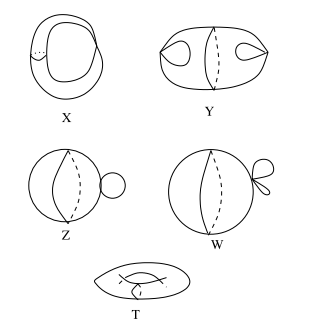
\includegraphics[max width=\textwidth]{2022-05-23 20_49_52-topology_merge.png}
%%%%%%%%%%%%%%%%%%%%%%%%%%%%%%%%%%%%%%%%%%%%%%%%%%%%%%%%%%%%%%%%%%%%%%%%%%%%%%%%%%%%%%%%%%%%%%%%%%%%%%%%%%%%%%%%%%%%%%%%
\newpage
%%%%%%%%%%%%%%%%%%%%%%%%%%%%%%%%%%%%%%%%%%%%%%%%%%%%%%%%%%%%%%%%%%%%%%%%%%%%%%%%%%%%%%%%%%%%%%%%%%%%%%%%%%%%%%%%%%%%%%%%
Let $D^{2}(r)=\left\{(x, y) \in \mathbb{R}^{2} \mid x^{2}+y^{2} \leq r^{2}\right\}$. Prove that if $f: D^{2}(1) \rightarrow \mathbb{R}$ is continuous then there exists $\bar{f}: D^{2}(2) \rightarrow \mathbb{R}$ continuous so that $\left.\bar{f}\right|_{D^{2}(1)}=f$.
%%%%%%%%%%%%%%%%%%%%%%%%%%%%%%%%%%%%%%%%%%%%%%%%%%%%%%%%%%%%%%%%%%%%%%%%%%%%%%%%%%%%%%%%%%%%%%%%%%%%%%%%%%%%%%%%%%%%%%%%
\newpage
%%%%%%%%%%%%%%%%%%%%%%%%%%%%%%%%%%%%%%%%%%%%%%%%%%%%%%%%%%%%%%%%%%%%%%%%%%%%%%%%%%%%%%%%%%%%%%%%%%%%%%%%%%%%%%%%%%%%%%%%
Prove that a subset of $\mathbb{R}$ in the standard topology is compact if and only if it is closed and bounded.
%%%%%%%%%%%%%%%%%%%%%%%%%%%%%%%%%%%%%%%%%%%%%%%%%%%%%%%%%%%%%%%%%%%%%%%%%%%%%%%%%%%%%%%%%%%%%%%%%%%%%%%%%%%%%%%%%%%%%%%%
\newpage
%%%%%%%%%%%%%%%%%%%%%%%%%%%%%%%%%%%%%%%%%%%%%%%%%%%%%%%%%%%%%%%%%%%%%%%%%%%%%%%%%%%%%%%%%%%%%%%%%%%%%%%%%%%%%%%%%%%%%%%%
%%%%%%%%%%%%%%%%%%%%%%%%%%%%%%%%%%%%%%%%%%%%%%%%%%%%%%%%%%%%%%%%%%%%%%%%%%%%%%%%%%%%%%%%%%%%%%%%%%%%%%%%%%%%%%%%%%%%%%%%
\newpage
%%%%%%%%%%%%%%%%%%%%%%%%%%%%%%%%%%%%%%%%%%%%%%%%%%%%%%%%%%%%%%%%%%%%%%%%%%%%%%%%%%%%%%%%%%%%%%%%%%%%%%%%%%%%%%%%%%%%%%%%
Let $M_{n}(\mathbb{R})=\mathbb{R}^{n^{2}}$ in the standard smooth structure. Here we are viewing $\mathbb{R}^{n^{2}}$ as $n \times n$-matrices with real coefficients.
(a) Prove that matrix multiplication,
$$
\mu: M_{n}(\mathbb{R}) \times M_{n}(\mathbb{R}) \rightarrow M_{n}(\mathbb{R})
$$
is a smooth map.

(b) Prove that the domain of definition of the matrix inverse $\iota$ is an open subset of $M_{n}(\mathbb{R})$, and that on its domain $G l_{n}(\mathbb{R})$, the matrix inverse $\iota: G l_{n}(\mathbb{R}) \rightarrow G l_{n}(\mathbb{R})$ is a smooth map.

(c) Prove that $G L_{n}(\mathbb{R})$ is a Lie group.

(d) What is the tangent space at the identity?

(e) How many connected components does $G L_{n}(\mathbb{R})$ have?
%%%%%%%%%%%%%%%%%%%%%%%%%%%%%%%%%%%%%%%%%%%%%%%%%%%%%%%%%%%%%%%%%%%%%%%%%%%%%%%%%%%%%%%%%%%%%%%%%%%%%%%%%%%%%%%%%%%%%%%%
\newpage
%%%%%%%%%%%%%%%%%%%%%%%%%%%%%%%%%%%%%%%%%%%%%%%%%%%%%%%%%%%%%%%%%%%%%%%%%%%%%%%%%%%%%%%%%%%%%%%%%%%%%%%%%%%%%%%%%%%%%%%%
Let $F \subset \mathbb{R}^{3}$ be a compact, oriented regular submanifold of dimension 2. Suppose that the boundary of $F$ is
$$
\partial F=\left\{(x, y, z) \in \mathbb{R}^{3} \mid z=0 \text { and either } x^{2}+y^{2}=1 \text { or } x^{2}+y^{2}=4\right\} .
$$
Furthermore looking down on $\partial F$ from above the $x y$-plane the smaller circle is oriented clockwise and the larger circle is oriented counterclockwise. Compute
$$
\int_{F} d x \wedge d y+d z \wedge d x+d z \wedge d y .
$$
%%%%%%%%%%%%%%%%%%%%%%%%%%%%%%%%%%%%%%%%%%%%%%%%%%%%%%%%%%%%%%%%%%%%%%%%%%%%%%%%%%%%%%%%%%%%%%%%%%%%%%%%%%%%%%%%%%%%%%%%
\newpage
%%%%%%%%%%%%%%%%%%%%%%%%%%%%%%%%%%%%%%%%%%%%%%%%%%%%%%%%%%%%%%%%%%%%%%%%%%%%%%%%%%%%%%%%%%%%%%%%%%%%%%%%%%%%%%%%%%%%%%%%
Going back to the map $F: \mathbb{R} P(2) \rightarrow \mathbb{R}^{3}$ from problem 1 of Part A,
(a) Display the standard smooth atlas for $\mathbb{R} P(2)$ and check at least one coordinate change is smooth.

(b) Show that $F: \mathbb{R} P(2) \rightarrow \mathbb{R}^{3}$ is smooth with respect to the standard smooth structures on $\mathbb{R} P(2)$ and $\mathbb{R}^{3}$.

(c) Can you find a point $[x, y, z] \in \mathbb{R} P(2)$ where $F_{*}: T_{[x, y, z]} \mathbb{R} P(2) \rightarrow$ $T_{F([x, y, z])} \mathbb{R}^{3}$ is not injective?
%%%%%%%%%%%%%%%%%%%%%%%%%%%%%%%%%%%%%%%%%%%%%%%%%%%%%%%%%%%%%%%%%%%%%%%%%%%%%%%%%%%%%%%%%%%%%%%%%%%%%%%%%%%%%%%%%%%%%%%%
\newpage
%%%%%%%%%%%%%%%%%%%%%%%%%%%%%%%%%%%%%%%%%%%%%%%%%%%%%%%%%%%%%%%%%%%%%%%%%%%%%%%%%%%%%%%%%%%%%%%%%%%%%%%%%%%%%%%%%%%%%%%%
Let
$$
S^{3}=\left\{(x, y, z, w) \in \mathbb{R}^{4} \mid x^{2}+y^{2}+z^{2}+w^{2}=1\right\}
$$
(a) Prove that $S^{3}$ is a regular submanifold of $\mathbb{R}^{4}$ in the standard smooth structure on $\mathbb{R}^{4}$.

(b) Characterize the tangent space to $S^{3}$ at an arbitrary point $(x, y, z, w) \in$ $S^{3}$.

(c) Can $S^{3}$ be smoothly embedded in $\mathbb{R}^{3}$ in the standard smooth structure?
%%%%%%%%%%%%%%%%%%%%%%%%%%%%%%%%%%%%%%%%%%%%%%%%%%%%%%%%%%%%%%%%%%%%%%%%%%%%%%%%%%%%%%%%%%%%%%%%%%%%%%%%%%%%%%%%%%%%%%%%
\newpage
%%%%%%%%%%%%%%%%%%%%%%%%%%%%%%%%%%%%%%%%%%%%%%%%%%%%%%%%%%%%%%%%%%%%%%%%%%%%%%%%%%%%%%%%%%%%%%%%%%%%%%%%%%%%%%%%%%%%%%%%
Let $T^{2}=S^{1} \times S^{1}$. Without obsessing to much on smooth structure, compute the De Rham cohomology of $T^{2}$. Justify your computation, stating any theorems you are using along the way.
%%%%%%%%%%%%%%%%%%%%%%%%%%%%%%%%%%%%%%%%%%%%%%%%%%%%%%%%%%%%%%%%%%%%%%%%%%%%%%%%%%%%%%%%%%%%%%%%%%%%%%%%%%%%%%%%%%%%%%%%
\newpage
%%%%%%%%%%%%%%%%%%%%%%%%%%%%%%%%%%%%%%%%%%%%%%%%%%%%%%%%%%%%%%%%%%%%%%%%%%%%%%%%%%%%%%%%%%%%%%%%%%%%%%%%%%%%%%%%%%%%%%%%
Recalling $S^{3}$ from Exercise 4 .
(a) Prove that the $\operatorname{maps} X(x, y, z, w)=(-y, x,-w, z) \in \mathbb{R}^{4}$ and $Y(x, y, z, w)=(-z,-w, x, y)$ define smooth vector fields on $S^{3}$.
(b) Compute their Lie bracket. Justify your computation.
%%%%%%%%%%%%%%%%%%%%%%%%%%%%%%%%%%%%%%%%%%%%%%%%%%%%%%%%%%%%%%%%%%%%%%%%%%%%%%%%%%%%%%%%%%%%%%%%%%%%%%%%%%%%%%%%%%%%%%%%
\newpage
%%%%%%%%%%%%%%%%%%%%%%%%%%%%%%%%%%%%%%%%%%%%%%%%%%%%%%%%%%%%%%%%%%%%%%%%%%%%%%%%%%%%%%%%%%%%%%%%%%%%%%%%%%%%%%%%%%%%%%%%
Prove that any open cover of a compact metric space has a Lebesgue number. That is if $(X, d)$ is a compact metric space and $\left\{U_{\alpha}\right\}_{\alpha \in A}$ is a covering of $X$ by open sets, there exists $\epsilon>0$ so that if $S \subset X$ has $\operatorname{diam}(S)<\epsilon$ then there exists $\alpha$ so that $S \subset U_{\alpha}$.
%%%%%%%%%%%%%%%%%%%%%%%%%%%%%%%%%%%%%%%%%%%%%%%%%%%%%%%%%%%%%%%%%%%%%%%%%%%%%%%%%%%%%%%%%%%%%%%%%%%%%%%%%%%%%%%%%%%%%%%%
\newpage
%%%%%%%%%%%%%%%%%%%%%%%%%%%%%%%%%%%%%%%%%%%%%%%%%%%%%%%%%%%%%%%%%%%%%%%%%%%%%%%%%%%%%%%%%%%%%%%%%%%%%%%%%%%%%%%%%%%%%%%%
Suppose that $X$ is a compact topological space and $\mathrm{Y}$ is a topological space. Give $X \times Y$ the product topology. Suppose that $y \in Y$. Prove that if $X \times\{y\} \subset W \subset X \times Y$ and $W$ is open in $X \times Y$ that there exists $U \subset Y$ open so that
$$
X \times\{y\} \subset X \times U \subset W .
$$
%%%%%%%%%%%%%%%%%%%%%%%%%%%%%%%%%%%%%%%%%%%%%%%%%%%%%%%%%%%%%%%%%%%%%%%%%%%%%%%%%%%%%%%%%%%%%%%%%%%%%%%%%%%%%%%%%%%%%%%%
\newpage
%%%%%%%%%%%%%%%%%%%%%%%%%%%%%%%%%%%%%%%%%%%%%%%%%%%%%%%%%%%%%%%%%%%%%%%%%%%%%%%%%%%%%%%%%%%%%%%%%%%%%%%%%%%%%%%%%%%%%%%%
 Prove that if $A \subset B \subset \bar{A} \subset X$ where $X$ is a topological space, $\bar{A}$ is the closure of $A$ and $A$ and $B$ have the subspace topology from $X$. Prove that if $A$ is connected then so is $B$.
%%%%%%%%%%%%%%%%%%%%%%%%%%%%%%%%%%%%%%%%%%%%%%%%%%%%%%%%%%%%%%%%%%%%%%%%%%%%%%%%%%%%%%%%%%%%%%%%%%%%%%%%%%%%%%%%%%%%%%%%
\newpage
%%%%%%%%%%%%%%%%%%%%%%%%%%%%%%%%%%%%%%%%%%%%%%%%%%%%%%%%%%%%%%%%%%%%%%%%%%%%%%%%%%%%%%%%%%%%%%%%%%%%%%%%%%%%%%%%%%%%%%%%
 Let $X \subset \mathbb{R}^{3}$ be the union of the unit circle in the $x y$-plane with the $z$-axis. Compute the fundamental group of
$$
\mathbb{R}^{3}-X
$$
Explain any homotopies you are using with annotated pictures.
%%%%%%%%%%%%%%%%%%%%%%%%%%%%%%%%%%%%%%%%%%%%%%%%%%%%%%%%%%%%%%%%%%%%%%%%%%%%%%%%%%%%%%%%%%%%%%%%%%%%%%%%%%%%%%%%%%%%%%%%
\newpage
%%%%%%%%%%%%%%%%%%%%%%%%%%%%%%%%%%%%%%%%%%%%%%%%%%%%%%%%%%%%%%%%%%%%%%%%%%%%%%%%%%%%%%%%%%%%%%%%%%%%%%%%%%%%%%%%%%%%%%%%
Let $p: E \rightarrow B$ be a covering projection where $E$ and $B$ are path connected, locally path connected and Hausdorff. If $b_{0}, b_{1} \in B$ prove that there is a one-to-one correspondence between $p^{-1}\left(b_{0}\right)$ and $p^{-1}\left(b_{1}\right)$.
%%%%%%%%%%%%%%%%%%%%%%%%%%%%%%%%%%%%%%%%%%%%%%%%%%%%%%%%%%%%%%%%%%%%%%%%%%%%%%%%%%%%%%%%%%%%%%%%%%%%%%%%%%%%%%%%%%%%%%%%
\newpage
%%%%%%%%%%%%%%%%%%%%%%%%%%%%%%%%%%%%%%%%%%%%%%%%%%%%%%%%%%%%%%%%%%%%%%%%%%%%%%%%%%%%%%%%%%%%%%%%%%%%%%%%%%%%%%%%%%%%%%%%
Let $K$ be a simplicial complex that is a triangulation of $\mathbb{R} P(2)$ the real projective plane.
(a) Draw such a simplicial complex. I recommend that it be as simple as possible.
(b) Set up the simplicial chain complex of $K$, describing bases for the chain groups and boundary maps.
(c) Compute the homology of the real projective plane.
%%%%%%%%%%%%%%%%%%%%%%%%%%%%%%%%%%%%%%%%%%%%%%%%%%%%%%%%%%%%%%%%%%%%%%%%%%%%%%%%%%%%%%%%%%%%%%%%%%%%%%%%%%%%%%%%%%%%%%%%
\newpage
%%%%%%%%%%%%%%%%%%%%%%%%%%%%%%%%%%%%%%%%%%%%%%%%%%%%%%%%%%%%%%%%%%%%%%%%%%%%%%%%%%%%%%%%%%%%%%%%%%%%%%%%%%%%%%%%%%%%%%%%
(a) Define the notion of a vectorfield on a smooth manifold $M$.

(b) Define the flow of a vectorfield on a smooth manifold $M$

(c) Let $X$ be a vectorfield on $M$. A nice periodic orbit of $X$ is a smooth embedding $\gamma: S^{1} \rightarrow M$ of an integral curve of $X$. Construct a vectorfield on the torus $M=S^{1} \times S^{1}$ which has no periodic orbits.

%%%%%%%%%%%%%%%%%%%%%%%%%%%%%%%%%%%%%%%%%%%%%%%%%%%%%%%%%%%%%%%%%%%%%%%%%%%%%%%%%%%%%%%%%%%%%%%%%%%%%%%%%%%%%%%%%%%%%%%%
\newpage
%%%%%%%%%%%%%%%%%%%%%%%%%%%%%%%%%%%%%%%%%%%%%%%%%%%%%%%%%%%%%%%%%%%%%%%%%%%%%%%%%%%%%%%%%%%%%%%%%%%%%%%%%%%%%%%%%%%%%%%%
Suppose $\gamma: S^{1} \rightarrow \mathbb{R}^{2}$ is a smooth embedding. Compute the integral $\int_{\gamma} \theta$ when
$$
\theta=x y^{2} d x+x^{2} y d y
$$

%%%%%%%%%%%%%%%%%%%%%%%%%%%%%%%%%%%%%%%%%%%%%%%%%%%%%%%%%%%%%%%%%%%%%%%%%%%%%%%%%%%%%%%%%%%%%%%%%%%%%%%%%%%%%%%%%%%%%%%%
\newpage
%%%%%%%%%%%%%%%%%%%%%%%%%%%%%%%%%%%%%%%%%%%%%%%%%%%%%%%%%%%%%%%%%%%%%%%%%%%%%%%%%%%%%%%%%%%%%%%%%%%%%%%%%%%%%%%%%%%%%%%%
Prove that a covering space of a smooth manifold $M$ is a smooth map between smooth manifolds
%%%%%%%%%%%%%%%%%%%%%%%%%%%%%%%%%%%%%%%%%%%%%%%%%%%%%%%%%%%%%%%%%%%%%%%%%%%%%%%%%%%%%%%%%%%%%%%%%%%%%%%%%%%%%%%%%%%%%%%%
\newpage
%%%%%%%%%%%%%%%%%%%%%%%%%%%%%%%%%%%%%%%%%%%%%%%%%%%%%%%%%%%%%%%%%%%%%%%%%%%%%%%%%%%%%%%%%%%%%%%%%%%%%%%%%%%%%%%%%%%%%%%%
Suppose that $M$ is a connected smooth manifold and let $p \in M$ be a point. Prove that if $\pi_{1}(M, p)$ has no non-trivial subgroups of index 2 then $M$ is orientable.
%%%%%%%%%%%%%%%%%%%%%%%%%%%%%%%%%%%%%%%%%%%%%%%%%%%%%%%%%%%%%%%%%%%%%%%%%%%%%%%%%%%%%%%%%%%%%%%%%%%%%%%%%%%%%%%%%%%%%%%%
\newpage
%%%%%%%%%%%%%%%%%%%%%%%%%%%%%%%%%%%%%%%%%%%%%%%%%%%%%%%%%%%%%%%%%%%%%%%%%%%%%%%%%%%%%%%%%%%%%%%%%%%%%%%%%%%%%%%%%%%%%%%%
A nulhomotopy of a map $f: \Omega^{*}(M) \rightarrow \Omega^{*}(M)$ is a collection of maps
$$
H: \Omega^{k}(M) \rightarrow \Omega^{k-1}(M) \quad \text { where } k \geq 0
$$
which satisfy the equation
$$
f=d H+H d
$$
If $X$ is a smooth vectorfield on $M$ then find a nulhomotopy for the Lie derivative $\mathcal{L}_{X}: \Omega^{*}(M) \rightarrow \Omega^{*}(M)$ of differential forms with respect to $X$.
%%%%%%%%%%%%%%%%%%%%%%%%%%%%%%%%%%%%%%%%%%%%%%%%%%%%%%%%%%%%%%%%%%%%%%%%%%%%%%%%%%%%%%%%%%%%%%%%%%%%%%%%%%%%%%%%%%%%%%%%
\newpage
%%%%%%%%%%%%%%%%%%%%%%%%%%%%%%%%%%%%%%%%%%%%%%%%%%%%%%%%%%%%%%%%%%%%%%%%%%%%%%%%%%%%%%%%%%%%%%%%%%%%%%%%%%%%%%%%%%%%%%%%
Prove that if $M$ is an oriented smooth manifold then the boundary $\partial M$ is also oriented.
%%%%%%%%%%%%%%%%%%%%%%%%%%%%%%%%%%%%%%%%%%%%%%%%%%%%%%%%%%%%%%%%%%%%%%%%%%%%%%%%%%%%%%%%%%%%%%%%%%%%%%%%%%%%%%%%%%%%%%%%
\newpage
%%%%%%%%%%%%%%%%%%%%%%%%%%%%%%%%%%%%%%%%%%%%%%%%%%%%%%%%%%%%%%%%%%%%%%%%%%%%%%%%%%%%%%%%%%%%%%%%%%%%%%%%%%%%%%%%%%%%%%%%
   Prove that every compact Hausdorff space is normal. That is prove that if $A$ and $B$ are disjoint closed subsets of the compact Hausdorff space $X$, then there are open sets $U$ and $V$ so that $U \cap V=\emptyset$, with $A \subset U, B \subset V$.
%%%%%%%%%%%%%%%%%%%%%%%%%%%%%%%%%%%%%%%%%%%%%%%%%%%%%%%%%%%%%%%%%%%%%%%%%%%%%%%%%%%%%%%%%%%%%%%%%%%%%%%%%%%%%%%%%%%%%%%%
\newpage
%%%%%%%%%%%%%%%%%%%%%%%%%%%%%%%%%%%%%%%%%%%%%%%%%%%%%%%%%%%%%%%%%%%%%%%%%%%%%%%%%%%%%%%%%%%%%%%%%%%%%%%%%%%%%%%%%%%%%%%%
   Prove the Lebesgue number lemma. That is if $X$ is a compact metric space and $\mathcal{U}$ is an open cover of $X$, there exists $\epsilon>0$ so that if $D$ is any subset of $X$ having diameter less than or equal to $\epsilon$ then there exists $U \in \mathcal{U}$ with $D \subset U$.
%%%%%%%%%%%%%%%%%%%%%%%%%%%%%%%%%%%%%%%%%%%%%%%%%%%%%%%%%%%%%%%%%%%%%%%%%%%%%%%%%%%%%%%%%%%%%%%%%%%%%%%%%%%%%%%%%%%%%%%%
\newpage
%%%%%%%%%%%%%%%%%%%%%%%%%%%%%%%%%%%%%%%%%%%%%%%%%%%%%%%%%%%%%%%%%%%%%%%%%%%%%%%%%%%%%%%%%%%%%%%%%%%%%%%%%%%%%%%%%%%%%%%%
   Prove that if $X$ and $Y$ are connected topological spaces then $X \times Y$ is connected.
%%%%%%%%%%%%%%%%%%%%%%%%%%%%%%%%%%%%%%%%%%%%%%%%%%%%%%%%%%%%%%%%%%%%%%%%%%%%%%%%%%%%%%%%%%%%%%%%%%%%%%%%%%%%%%%%%%%%%%%%
\newpage
%%%%%%%%%%%%%%%%%%%%%%%%%%%%%%%%%%%%%%%%%%%%%%%%%%%%%%%%%%%%%%%%%%%%%%%%%%%%%%%%%%%%%%%%%%%%%%%%%%%%%%%%%%%%%%%%%%%%%%%%
   Give an example of a space that is connected but not path connected. Justify your answer.
%%%%%%%%%%%%%%%%%%%%%%%%%%%%%%%%%%%%%%%%%%%%%%%%%%%%%%%%%%%%%%%%%%%%%%%%%%%%%%%%%%%%%%%%%%%%%%%%%%%%%%%%%%%%%%%%%%%%%%%%
\newpage
%%%%%%%%%%%%%%%%%%%%%%%%%%%%%%%%%%%%%%%%%%%%%%%%%%%%%%%%%%%%%%%%%%%%%%%%%%%%%%%%%%%%%%%%%%%%%%%%%%%%%%%%%%%%%%%%%%%%%%%%
   Let $\mathbb{R} P(n)$ be the quotient space obtained from $\mathbb{R}^{n+1}-\{0\}$ under the equivalence relation, that two points are equivalent if they are scalar multiples of one another. Prove that $\mathbb{R} P(n)$ is second countable, Hausdorff and compact.
%%%%%%%%%%%%%%%%%%%%%%%%%%%%%%%%%%%%%%%%%%%%%%%%%%%%%%%%%%%%%%%%%%%%%%%%%%%%%%%%%%%%%%%%%%%%%%%%%%%%%%%%%%%%%%%%%%%%%%%%
\newpage
%%%%%%%%%%%%%%%%%%%%%%%%%%%%%%%%%%%%%%%%%%%%%%%%%%%%%%%%%%%%%%%%%%%%%%%%%%%%%%%%%%%%%%%%%%%%%%%%%%%%%%%%%%%%%%%%%%%%%%%%
a. Suppose that $X$ is compact and $Y$ is Hausdorff. Prove that every one-to-one, onto, continuous map $f: X \rightarrow Y$ is a homeomorphism.
b. Suppose that $X$ is compact and nonempty, and $Y$ is Hausdorff and connected. Prove that any continuous, open map $f: X \rightarrow Y$ is onto.
%%%%%%%%%%%%%%%%%%%%%%%%%%%%%%%%%%%%%%%%%%%%%%%%%%%%%%%%%%%%%%%%%%%%%%%%%%%%%%%%%%%%%%%%%%%%%%%%%%%%%%%%%%%%%%%%%%%%%%%%
\newpage
%%%%%%%%%%%%%%%%%%%%%%%%%%%%%%%%%%%%%%%%%%%%%%%%%%%%%%%%%%%%%%%%%%%%%%%%%%%%%%%%%%%%%%%%%%%%%%%%%%%%%%%%%%%%%%%%%%%%%%%%
a. Define $T_{p} M$ where $M$ is a smooth manifold and $p \in M$.
b. If $F: M \rightarrow N$ is a smooth map of smooth manifolds define $F_{*}$ : $T_{p} M \rightarrow T_{F(p)} N$.
c. Prove the chain rule, that is if $F: M \rightarrow N$ and $G: N \rightarrow P$ are smooth maps of smooth manifolds then $(G \circ F)_{*}=G_{*} \circ F_{*}$.
%%%%%%%%%%%%%%%%%%%%%%%%%%%%%%%%%%%%%%%%%%%%%%%%%%%%%%%%%%%%%%%%%%%%%%%%%%%%%%%%%%%%%%%%%%%%%%%%%%%%%%%%%%%%%%%%%%%%%%%%
\newpage
%%%%%%%%%%%%%%%%%%%%%%%%%%%%%%%%%%%%%%%%%%%%%%%%%%%%%%%%%%%%%%%%%%%%%%%%%%%%%%%%%%%%%%%%%%%%%%%%%%%%%%%%%%%%%%%%%%%%%%%%
a. Prove that the hyperboloid $H$ of points in $\mathbb{R}^{3}$ that satisfy

$$
x^{2}+y^{2}-z^{2}=1
$$
is a smooth submanifold of $\mathbb{R}^{3}$.

b. Let $p: H \rightarrow \mathbb{R}^{2}$ be the restriction of orthogonal projection to the $x z$-plane to $H$. What are the regular values and critical values of $p$ ? Justify your answer.

%%%%%%%%%%%%%%%%%%%%%%%%%%%%%%%%%%%%%%%%%%%%%%%%%%%%%%%%%%%%%%%%%%%%%%%%%%%%%%%%%%%%%%%%%%%%%%%%%%%%%%%%%%%%%%%%%%%%%%%%
\newpage
%%%%%%%%%%%%%%%%%%%%%%%%%%%%%%%%%%%%%%%%%%%%%%%%%%%%%%%%%%%%%%%%%%%%%%%%%%%%%%%%%%%%%%%%%%%%%%%%%%%%%%%%%%%%%%%%%%%%%%%%
a. Define Lie group.

b. Let $S L_{n} \mathbb{R}$ denote $n \times n$-matrices with real entries of determinant 1 . Prove that $S L_{n} \mathbb{R}$ is a Lie group.

c. What is the tangent space of $S L_{n} \mathbb{R}$ at the identity?

%%%%%%%%%%%%%%%%%%%%%%%%%%%%%%%%%%%%%%%%%%%%%%%%%%%%%%%%%%%%%%%%%%%%%%%%%%%%%%%%%%%%%%%%%%%%%%%%%%%%%%%%%%%%%%%%%%%%%%%%
\newpage
%%%%%%%%%%%%%%%%%%%%%%%%%%%%%%%%%%%%%%%%%%%%%%%%%%%%%%%%%%%%%%%%%%%%%%%%%%%%%%%%%%%%%%%%%%%%%%%%%%%%%%%%%%%%%%%%%%%%%%%%
State and prove the local immersion theorem.
%%%%%%%%%%%%%%%%%%%%%%%%%%%%%%%%%%%%%%%%%%%%%%%%%%%%%%%%%%%%%%%%%%%%%%%%%%%%%%%%%%%%%%%%%%%%%%%%%%%%%%%%%%%%%%%%%%%%%%%%
\newpage
%%%%%%%%%%%%%%%%%%%%%%%%%%%%%%%%%%%%%%%%%%%%%%%%%%%%%%%%%%%%%%%%%%%%%%%%%%%%%%%%%%%%%%%%%%%%%%%%%%%%%%%%%%%%%%%%%%%%%%%%
a. If $c: I^{n} \rightarrow M$ is a singular cube, define $\partial c$.
b. Give a list of properties of the exterior derivative that uniquely determines it on any smooth manifold.
c. State the fundamental theorem of calculus.
d. Check that the fundamental theorem of calculus is true by evaluating both sides of the equation for the following example. Use the singular cube $c: I^{2} \rightarrow \mathbb{R}^{2}$ given by
$$
c(s, t)=(s \cos 2 \pi t, s \sin 2 \pi t)
$$
and the form $\omega=x \mathrm{~d} y-y \mathrm{~d} x$. Justify the steps of your computation.

%%%%%%%%%%%%%%%%%%%%%%%%%%%%%%%%%%%%%%%%%%%%%%%%%%%%%%%%%%%%%%%%%%%%%%%%%%%%%%%%%%%%%%%%%%%%%%%%%%%%%%%%%%%%%%%%%%%%%%%%
\newpage
%%%%%%%%%%%%%%%%%%%%%%%%%%%%%%%%%%%%%%%%%%%%%%%%%%%%%%%%%%%%%%%%%%%%%%%%%%%%%%%%%%%%%%%%%%%%%%%%%%%%%%%%%%%%%%%%%%%%%%%%
a. Define smooth manifold. On your way you should define all the terms you need for the second part of the question.

b. Prove that each $C^{\infty}$-compatible atlas on a manifold is contained in a unique differentiable structure.
%%%%%%%%%%%%%%%%%%%%%%%%%%%%%%%%%%%%%%%%%%%%%%%%%%%%%%%%%%%%%%%%%%%%%%%%%%%%%%%%%%%%%%%%%%%%%%%%%%%%%%%%%%%%%%%%%%%%%%%%
\newpage
%%%%%%%%%%%%%%%%%%%%%%%%%%%%%%%%%%%%%%%%%%%%%%%%%%%%%%%%%%%%%%%%%%%%%%%%%%%%%%%%%%%%%%%%%%%%%%%%%%%%%%%%%%%%%%%%%%%%%%%%
   Suppose that $X$ and $Y$ are connected, nonempty topological spaces. Prove that $X \times Y$ is connected.
%%%%%%%%%%%%%%%%%%%%%%%%%%%%%%%%%%%%%%%%%%%%%%%%%%%%%%%%%%%%%%%%%%%%%%%%%%%%%%%%%%%%%%%%%%%%%%%%%%%%%%%%%%%%%%%%%%%%%%%%
\newpage
%%%%%%%%%%%%%%%%%%%%%%%%%%%%%%%%%%%%%%%%%%%%%%%%%%%%%%%%%%%%%%%%%%%%%%%%%%%%%%%%%%%%%%%%%%%%%%%%%%%%%%%%%%%%%%%%%%%%%%%%
   Suppose that $X$ is a compact Hausdorff space and $A$ and $B$ are closed disjoint subsets of $X$. Prove that there exists $U$ and $V$ open in $X$ with $U \cap V=\emptyset$ and $A \subset U, B \subset V$. That is, prove that $X$ is normal.
%%%%%%%%%%%%%%%%%%%%%%%%%%%%%%%%%%%%%%%%%%%%%%%%%%%%%%%%%%%%%%%%%%%%%%%%%%%%%%%%%%%%%%%%%%%%%%%%%%%%%%%%%%%%%%%%%%%%%%%%
\newpage
%%%%%%%%%%%%%%%%%%%%%%%%%%%%%%%%%%%%%%%%%%%%%%%%%%%%%%%%%%%%%%%%%%%%%%%%%%%%%%%%%%%%%%%%%%%%%%%%%%%%%%%%%%%%%%%%%%%%%%%%
   Suppose that $X$ is Hausdorff and $f, g: Y \rightarrow X$ are continuous. Prove that the set $\{y \in Y \mid f(y)=g(y)\}$ is closed.
%%%%%%%%%%%%%%%%%%%%%%%%%%%%%%%%%%%%%%%%%%%%%%%%%%%%%%%%%%%%%%%%%%%%%%%%%%%%%%%%%%%%%%%%%%%%%%%%%%%%%%%%%%%%%%%%%%%%%%%%
\newpage
%%%%%%%%%%%%%%%%%%%%%%%%%%%%%%%%%%%%%%%%%%%%%%%%%%%%%%%%%%%%%%%%%%%%%%%%%%%%%%%%%%%%%%%%%%%%%%%%%%%%%%%%%%%%%%%%%%%%%%%%
   A space is separable if it has a countable dense subset. Prove that a topological space is separable if it is second countable, and that a metric space is second countable if it is separable. There are two things to prove here.
%%%%%%%%%%%%%%%%%%%%%%%%%%%%%%%%%%%%%%%%%%%%%%%%%%%%%%%%%%%%%%%%%%%%%%%%%%%%%%%%%%%%%%%%%%%%%%%%%%%%%%%%%%%%%%%%%%%%%%%%
\newpage
%%%%%%%%%%%%%%%%%%%%%%%%%%%%%%%%%%%%%%%%%%%%%%%%%%%%%%%%%%%%%%%%%%%%%%%%%%%%%%%%%%%%%%%%%%%%%%%%%%%%%%%%%%%%%%%%%%%%%%%%
   Prove that if $X$ is compact, $Y$ is Hausdorff and $f: X \rightarrow Y$ is one to one, onto and continuous, then $f$ is a homeomorphism. 6. Suppose that $p: X \rightarrow Z$ is a quotient map and $f: X \rightarrow Y$ is continuous. Prove that there exists a continuous map $\bar{f}: Z \rightarrow Y$ with $\bar{f} \circ p=f$ if and only if for every $x_{1}, x_{2}$ with $p\left(x_{1}\right)=p\left(x_{2}\right)$ it is the case that $f\left(x_{1}\right)=f\left(x_{2}\right)$.
%%%%%%%%%%%%%%%%%%%%%%%%%%%%%%%%%%%%%%%%%%%%%%%%%%%%%%%%%%%%%%%%%%%%%%%%%%%%%%%%%%%%%%%%%%%%%%%%%%%%%%%%%%%%%%%%%%%%%%%%
\newpage
%%%%%%%%%%%%%%%%%%%%%%%%%%%%%%%%%%%%%%%%%%%%%%%%%%%%%%%%%%%%%%%%%%%%%%%%%%%%%%%%%%%%%%%%%%%%%%%%%%%%%%%%%%%%%%%%%%%%%%%%
 Prove the local immersion theorem. If $F: M \rightarrow N$ is a smooth map of smooth manifolds and $d F$ (the differential of $F$ ) is injective at $P$ then there are local coordinates $(U, \phi)$ at $P$ and $(V, \psi)$ at $F(P)$ so that $F(U) \subset V$ and.

$$
\psi \circ F \circ \phi^{-1}\left(x^{1}, \ldots, x^{m}\right)=\left(x^{1}, \ldots, x^{m}, 0, \ldots, 0\right)
$$
%%%%%%%%%%%%%%%%%%%%%%%%%%%%%%%%%%%%%%%%%%%%%%%%%%%%%%%%%%%%%%%%%%%%%%%%%%%%%%%%%%%%%%%%%%%%%%%%%%%%%%%%%%%%%%%%%%%%%%%%
\newpage
%%%%%%%%%%%%%%%%%%%%%%%%%%%%%%%%%%%%%%%%%%%%%%%%%%%%%%%%%%%%%%%%%%%%%%%%%%%%%%%%%%%%%%%%%%%%%%%%%%%%%%%%%%%%%%%%%%%%%%%%
 Let $O(n)$ denote the set of $n \times n$ matrices with real entries, $A$ so that $A A^{t}=I d$. Prove that $O(n)$ is a Lie group, and identify the tangent space at the identity.
%%%%%%%%%%%%%%%%%%%%%%%%%%%%%%%%%%%%%%%%%%%%%%%%%%%%%%%%%%%%%%%%%%%%%%%%%%%%%%%%%%%%%%%%%%%%%%%%%%%%%%%%%%%%%%%%%%%%%%%%
\newpage
%%%%%%%%%%%%%%%%%%%%%%%%%%%%%%%%%%%%%%%%%%%%%%%%%%%%%%%%%%%%%%%%%%%%%%%%%%%%%%%%%%%%%%%%%%%%%%%%%%%%%%%%%%%%%%%%%%%%%%%%
 Let $T^{2}$ be the subset $\mathbb{R}^{3}$ that is the result of rotating the circle in the $y z$ plane of radius 1 centered at $(0,2,0)$ about the $z$-axis. It may be useful to note that $T^{2}$ is the set of points in 3-space satisfying the equation $\left(\left(x^{2}+y^{2}\right)^{1 / 2}-2\right)^{2}+z^{2}=1 .$
\begin{itemize}
  \item Prove that $T^{2}$ is a smooth 2-manifold.

  \item Let $p: T^{2} \rightarrow \mathbb{R}^{2}$ be the restriction of $p: \mathbb{R}^{3} \rightarrow \mathbb{R}^{2}$ given by $p(x, y, z)=(x, y)$. Identify the regular values of $p: T^{2} \rightarrow \mathbb{R}^{2}$.

\end{itemize}
%%%%%%%%%%%%%%%%%%%%%%%%%%%%%%%%%%%%%%%%%%%%%%%%%%%%%%%%%%%%%%%%%%%%%%%%%%%%%%%%%%%%%%%%%%%%%%%%%%%%%%%%%%%%%%%%%%%%%%%%
\newpage
%%%%%%%%%%%%%%%%%%%%%%%%%%%%%%%%%%%%%%%%%%%%%%%%%%%%%%%%%%%%%%%%%%%%%%%%%%%%%%%%%%%%%%%%%%%%%%%%%%%%%%%%%%%%%%%%%%%%%%%%
 Let $S^{2}$ be the unit sphere centered at the origin in $\mathbb{R}^{3}$ given the standard orientation as the boundary of the ball. Let $\omega$ be the two form on $S^{2}$ that is the restriction of $x d y \wedge d z-y d x \wedge d z+z d x \wedge d y$ to the sphere. Compute

$$
\int_{S^{2}} \omega
$$

%%%%%%%%%%%%%%%%%%%%%%%%%%%%%%%%%%%%%%%%%%%%%%%%%%%%%%%%%%%%%%%%%%%%%%%%%%%%%%%%%%%%%%%%%%%%%%%%%%%%%%%%%%%%%%%%%%%%%%%%
\newpage
%%%%%%%%%%%%%%%%%%%%%%%%%%%%%%%%%%%%%%%%%%%%%%%%%%%%%%%%%%%%%%%%%%%%%%%%%%%%%%%%%%%%%%%%%%%%%%%%%%%%%%%%%%%%%%%%%%%%%%%%
Let $M$ be a smooth manifold.

\begin{itemize}
  \item Given $P \in M$ define $T_{P} M$.

  \item Define smooth vector field on $M$. - If $X$ and $Y$ are smooth vector fields on $M$ define $[X, Y]$.

  \item Compute $[X, Y]$ where $X=x \frac{\partial}{\partial y}+\frac{\partial}{\partial x}$ and $Y=\frac{\partial}{\partial x}+\frac{\partial}{\partial y}$ are vector fields on the plane.

\end{itemize}
%%%%%%%%%%%%%%%%%%%%%%%%%%%%%%%%%%%%%%%%%%%%%%%%%%%%%%%%%%%%%%%%%%%%%%%%%%%%%%%%%%%%%%%%%%%%%%%%%%%%%%%%%%%%%%%%%%%%%%%%
\newpage
%%%%%%%%%%%%%%%%%%%%%%%%%%%%%%%%%%%%%%%%%%%%%%%%%%%%%%%%%%%%%%%%%%%%%%%%%%%%%%%%%%%%%%%%%%%%%%%%%%%%%%%%%%%%%%%%%%%%%%%%
 Suppose that $M$ and $N$ are smooth manifolds. Give $M \times N$ the structure of a smooth manifold by producing a compatible atlas. Prove that your atlas is compatible.
%%%%%%%%%%%%%%%%%%%%%%%%%%%%%%%%%%%%%%%%%%%%%%%%%%%%%%%%%%%%%%%%%%%%%%%%%%%%%%%%%%%%%%%%%%%%%%%%%%%%%%%%%%%%%%%%%%%%%%%%
\newpage
%%%%%%%%%%%%%%%%%%%%%%%%%%%%%%%%%%%%%%%%%%%%%%%%%%%%%%%%%%%%%%%%%%%%%%%%%%%%%%%%%%%%%%%%%%%%%%%%%%%%%%%%%%%%%%%%%%%%%%%%
A1) Suppose that $X$ and $Y$ are connected, prove that $X \times Y$ is connected.
%%%%%%%%%%%%%%%%%%%%%%%%%%%%%%%%%%%%%%%%%%%%%%%%%%%%%%%%%%%%%%%%%%%%%%%%%%%%%%%%%%%%%%%%%%%%%%%%%%%%%%%%%%%%%%%%%%%%%%%%
\newpage
%%%%%%%%%%%%%%%%%%%%%%%%%%%%%%%%%%%%%%%%%%%%%%%%%%%%%%%%%%%%%%%%%%%%%%%%%%%%%%%%%%%%%%%%%%%%%%%%%%%%%%%%%%%%%%%%%%%%%%%%
A2) Tube Lemma Suppose that $X$ is compact and $X \times\{y\} \subset U$ where $U \subset X \times Y$ is open. Prove that there exists $W \subset Y$ open so that $X \times\{y\} \subset X \times W \subset U$
%%%%%%%%%%%%%%%%%%%%%%%%%%%%%%%%%%%%%%%%%%%%%%%%%%%%%%%%%%%%%%%%%%%%%%%%%%%%%%%%%%%%%%%%%%%%%%%%%%%%%%%%%%%%%%%%%%%%%%%%
\newpage
%%%%%%%%%%%%%%%%%%%%%%%%%%%%%%%%%%%%%%%%%%%%%%%%%%%%%%%%%%%%%%%%%%%%%%%%%%%%%%%%%%%%%%%%%%%%%%%%%%%%%%%%%%%%%%%%%%%%%%%%
A3) Suppose that $X$ is compact and $Y$ is Hausdorff. Prove that if $f: X \rightarrow Y$ is continuous then $f(X)$ is closed. This proof should be from definitions.
%%%%%%%%%%%%%%%%%%%%%%%%%%%%%%%%%%%%%%%%%%%%%%%%%%%%%%%%%%%%%%%%%%%%%%%%%%%%%%%%%%%%%%%%%%%%%%%%%%%%%%%%%%%%%%%%%%%%%%%%
\newpage
%%%%%%%%%%%%%%%%%%%%%%%%%%%%%%%%%%%%%%%%%%%%%%%%%%%%%%%%%%%%%%%%%%%%%%%%%%%%%%%%%%%%%%%%%%%%%%%%%%%%%%%%%%%%%%%%%%%%%%%%
A4) Let $\mathbb{R} P(n)$ be the quotient space from $\mathbb{R}^{n+1}-\{\overrightarrow{0}\}$ by the equivalence relation $\left(x_{0}, \ldots, x_{n}\right) \sim\left(x_{0}^{\prime}, \ldots, x_{n}^{\prime}\right)$ if there exists $\lambda \in \mathbb{R}$ so that
$$
\lambda\left(x_{0}, \ldots, x_{n}\right)=\left(x_{0}^{\prime}, \ldots, x_{n}^{\prime}\right)
$$
a. Prove that the quotient map $q: \mathbb{R}^{n+1}-\{\overrightarrow{0}\} \rightarrow \mathbb{R} P(n)$ is open.

b. Prove that $\mathbb{R} P(n)$ is second countable.
%%%%%%%%%%%%%%%%%%%%%%%%%%%%%%%%%%%%%%%%%%%%%%%%%%%%%%%%%%%%%%%%%%%%%%%%%%%%%%%%%%%%%%%%%%%%%%%%%%%%%%%%%%%%%%%%%%%%%%%%
\newpage
%%%%%%%%%%%%%%%%%%%%%%%%%%%%%%%%%%%%%%%%%%%%%%%%%%%%%%%%%%%%%%%%%%%%%%%%%%%%%%%%%%%%%%%%%%%%%%%%%%%%%%%%%%%%%%%%%%%%%%%%
A5) Let $X$ be a topological space and let
$$
\Delta=\{(x, x) \in X \times X\} .
$$
Prove that $X$ is Hausdorff if and only if $\Delta \subset X \times X$ is closed.
%%%%%%%%%%%%%%%%%%%%%%%%%%%%%%%%%%%%%%%%%%%%%%%%%%%%%%%%%%%%%%%%%%%%%%%%%%%%%%%%%%%%%%%%%%%%%%%%%%%%%%%%%%%%%%%%%%%%%%%%
\newpage
%%%%%%%%%%%%%%%%%%%%%%%%%%%%%%%%%%%%%%%%%%%%%%%%%%%%%%%%%%%%%%%%%%%%%%%%%%%%%%%%%%%%%%%%%%%%%%%%%%%%%%%%%%%%%%%%%%%%%%%%
A6) Prove that if $X$ is compact, $Y$ is Hausdorff, and $f: X \rightarrow Y$ is continuous, one-to-one and onto then $f$ is a homeomorphism.
%%%%%%%%%%%%%%%%%%%%%%%%%%%%%%%%%%%%%%%%%%%%%%%%%%%%%%%%%%%%%%%%%%%%%%%%%%%%%%%%%%%%%%%%%%%%%%%%%%%%%%%%%%%%%%%%%%%%%%%%
\newpage
%%%%%%%%%%%%%%%%%%%%%%%%%%%%%%%%%%%%%%%%%%%%%%%%%%%%%%%%%%%%%%%%%%%%%%%%%%%%%%%%%%%%%%%%%%%%%%%%%%%%%%%%%%%%%%%%%%%%%%%%
B1) Prove that the sphere $S^{2}=\left\{(x, y, z) \in \mathbb{R}^{3}: x^{2}+y^{2}+z^{2}=1\right\}$ is a smooth manifold by exhibiting charts. Carefully calculate one transition map and its derivative to explain why the transition map is a diffeomorphism.
%%%%%%%%%%%%%%%%%%%%%%%%%%%%%%%%%%%%%%%%%%%%%%%%%%%%%%%%%%%%%%%%%%%%%%%%%%%%%%%%%%%%%%%%%%%%%%%%%%%%%%%%%%%%%%%%%%%%%%%%
\newpage
%%%%%%%%%%%%%%%%%%%%%%%%%%%%%%%%%%%%%%%%%%%%%%%%%%%%%%%%%%%%%%%%%%%%%%%%%%%%%%%%%%%%%%%%%%%%%%%%%%%%%%%%%%%%%%%%%%%%%%%%
B2) Prove that the surface $H=\left\{(x, y, z) \in \mathbb{R}^{3}: x^{2}-y^{2}+z^{2}=3\right\}$ is a smooth manifold by showing $H$ is the pre-image of a regular value of a smooth map.

Justify your various claims.
%%%%%%%%%%%%%%%%%%%%%%%%%%%%%%%%%%%%%%%%%%%%%%%%%%%%%%%%%%%%%%%%%%%%%%%%%%%%%%%%%%%%%%%%%%%%%%%%%%%%%%%%%%%%%%%%%%%%%%%%
\newpage
%%%%%%%%%%%%%%%%%%%%%%%%%%%%%%%%%%%%%%%%%%%%%%%%%%%%%%%%%%%%%%%%%%%%%%%%%%%%%%%%%%%%%%%%%%%%%%%%%%%%%%%%%%%%%%%%%%%%%%%%
B3) Let $A=\left\{(x, y, z) \in \mathbb{R}^{3}: z=2 x+3 y\right\}$ and let $B=$ the $z-$ axis.

Prove $A$ and $B$ meet transversally.
%%%%%%%%%%%%%%%%%%%%%%%%%%%%%%%%%%%%%%%%%%%%%%%%%%%%%%%%%%%%%%%%%%%%%%%%%%%%%%%%%%%%%%%%%%%%%%%%%%%%%%%%%%%%%%%%%%%%%%%%
\newpage
%%%%%%%%%%%%%%%%%%%%%%%%%%%%%%%%%%%%%%%%%%%%%%%%%%%%%%%%%%%%%%%%%%%%%%%%%%%%%%%%%%%%%%%%%%%%%%%%%%%%%%%%%%%%%%%%%%%%%%%%
B4) Suppose $X, Y, Z$ are smooth manifolds, $f: X \rightarrow Y$ is a diffeomorphism, and $g: Y \rightarrow Z$ is a smooth map such that for some $y \in Y, d g_{y}: T_{y} Y \rightarrow T_{g(y)} Z$ is injective. Prove that for each $x \in f^{-1}(y), d_{x}(g \circ f)$ is injective.
%%%%%%%%%%%%%%%%%%%%%%%%%%%%%%%%%%%%%%%%%%%%%%%%%%%%%%%%%%%%%%%%%%%%%%%%%%%%%%%%%%%%%%%%%%%%%%%%%%%%%%%%%%%%%%%%%%%%%%%%
\newpage
%%%%%%%%%%%%%%%%%%%%%%%%%%%%%%%%%%%%%%%%%%%%%%%%%%%%%%%%%%%%%%%%%%%%%%%%%%%%%%%%%%%%%%%%%%%%%%%%%%%%%%%%%%%%%%%%%%%%%%%%
B5) Let $\mathcal{M}$ be the set of all $2 \times 2$ matrices (with real-number entries).

a. Let $\mathcal{M}_{0}=\{M \in \mathcal{M}: \operatorname{det}(M) \neq 0\}$. Explain how we can view $\mathcal{M}_{0}$ as a smooth manifold. Make sure to explain the dimension of $\mathcal{M}_{0}$.

b. Let $\mathcal{M}_{1}=\{M \in \mathcal{M}: \operatorname{det}(M)=1\}$. Explain how we can view $\mathcal{M}_{1}$ as a smooth manifold. Make sure to explain the dimension of $\mathcal{M}_{1}$.
%%%%%%%%%%%%%%%%%%%%%%%%%%%%%%%%%%%%%%%%%%%%%%%%%%%%%%%%%%%%%%%%%%%%%%%%%%%%%%%%%%%%%%%%%%%%%%%%%%%%%%%%%%%%%%%%%%%%%%%%
\newpage
%%%%%%%%%%%%%%%%%%%%%%%%%%%%%%%%%%%%%%%%%%%%%%%%%%%%%%%%%%%%%%%%%%%%%%%%%%%%%%%%%%%%%%%%%%%%%%%%%%%%%%%%%%%%%%%%%%%%%%%%
B6) Consider the following 1 -form on $\mathbb{R}^{3}$.
$$
\omega=x y d x+x d y+x d z
$$
(i) Calculate the 2 -form $d \omega$.

(ii) Show by explicit calculation that $d(d \omega)=0$.

(iii) Does there exist a 1-form $\alpha$ on $\mathbb{R}^{3}$ such that $d d \alpha=\left(x^{5} y^{3} z^{9}\right) d x \wedge d y \wedge d z ?$ (Do not try to find such $\alpha$; just state in one or two sentences why such a 1-form does or does not exist.)

%%%%%%%%%%%%%%%%%%%%%%%%%%%%%%%%%%%%%%%%%%%%%%%%%%%%%%%%%%%%%%%%%%%%%%%%%%%%%%%%%%%%%%%%%%%%%%%%%%%%%%%%%%%%%%%%%%%%%%%%
\newpage
%%%%%%%%%%%%%%%%%%%%%%%%%%%%%%%%%%%%%%%%%%%%%%%%%%%%%%%%%%%%%%%%%%%%%%%%%%%%%%%%%%%%%%%%%%%%%%%%%%%%%%%%%%%%%%%%%%%%%%%%
Let $\Sigma$ be an oriented closed surface of genus $g$. Consider the group action $\rho$ of $S_{g}$ on the $g$-fold product space $\Sigma \times \cdots \times \Sigma$ as
$$
\rho(\sigma):\left(x_{1}, \cdots, x_{g}\right) \mapsto\left(x_{\sigma(1)}, \cdots, x_{\sigma(g)}\right) .
$$
Consider the quotient space $\Sigma \times \cdots \times \Sigma / S_{g}$ which is denoted by $\operatorname{Sym}^{g}(\Sigma)$. Let $\alpha_{1}, \cdots, \alpha_{g}, \beta_{1}, \cdots, \beta_{g}$ be embedded, pairwise distinct circles in $\Sigma$. Consider subspaces of $\operatorname{Sym}^{g}(\Sigma)$
$$
\mathbb{T}_{\alpha}=\alpha_{1} \times \cdots \times \alpha_{g} \text { and } \mathbb{T}_{\beta}=\beta_{1} \times \cdots \times \beta_{g} .
$$
(a) What is the dimension of $\operatorname{Sym}^{g}(\Sigma)$ ?

(b) Describe the intersection $\mathbb{T}_{\alpha} \cap \mathbb{T}_{\beta}$.

%%%%%%%%%%%%%%%%%%%%%%%%%%%%%%%%%%%%%%%%%%%%%%%%%%%%%%%%%%%%%%%%%%%%%%%%%%%%%%%%%%%%%%%%%%%%%%%%%%%%%%%%%%%%%%%%%%%%%%%%
\newpage
%%%%%%%%%%%%%%%%%%%%%%%%%%%%%%%%%%%%%%%%%%%%%%%%%%%%%%%%%%%%%%%%%%%%%%%%%%%%%%%%%%%%%%%%%%%%%%%%%%%%%%%%%%%%%%%%%%%%%%%%
   Let $X \approx D^{2} \times S^{1}$ be an unknotted solid torus embedded in $S^{3}$. Let $T:=\partial X \approx S^{1} \times S^{1}$ and a meridian $\mu:=S^{1} \times\{\cdot\}$ and a longitude $\lambda:=\{\cdot\} \times S^{1}$. Let $\phi: T \rightarrow T$ be a diffeomorphism whose induced homomorphism $\phi_{*}: \pi_{1}(T) \rightarrow \pi_{1}(T)$ of the fundamental group takes the homotopy class $[\mu]$ to the homotopy class $p[\mu]+q[\lambda]$. The Lens space $L(p, q)$ is a closed manifold obtained from $S^{3}$ removing $T$ from $S^{3}$ and then gluing back $T$ using the diffeomorphism $\phi$. Find the fundamental group of the lens space $L(p, q)$.
%%%%%%%%%%%%%%%%%%%%%%%%%%%%%%%%%%%%%%%%%%%%%%%%%%%%%%%%%%%%%%%%%%%%%%%%%%%%%%%%%%%%%%%%%%%%%%%%%%%%%%%%%%%%%%%%%%%%%%%%
\newpage
%%%%%%%%%%%%%%%%%%%%%%%%%%%%%%%%%%%%%%%%%%%%%%%%%%%%%%%%%%%%%%%%%%%%%%%%%%%%%%%%%%%%%%%%%%%%%%%%%%%%%%%%%%%%%%%%%%%%%%%%
   Let $X \approx D^{2} \backslash\{p, q, r\}$ be a trice-punctured disk. Find a 2 -fold cover $\tilde{X}$ of $X$, and describe how the covering transformation group acts on $\tilde{X}$.
%%%%%%%%%%%%%%%%%%%%%%%%%%%%%%%%%%%%%%%%%%%%%%%%%%%%%%%%%%%%%%%%%%%%%%%%%%%%%%%%%%%%%%%%%%%%%%%%%%%%%%%%%%%%%%%%%%%%%%%%
\newpage
%%%%%%%%%%%%%%%%%%%%%%%%%%%%%%%%%%%%%%%%%%%%%%%%%%%%%%%%%%%%%%%%%%%%%%%%%%%%%%%%%%%%%%%%%%%%%%%%%%%%%%%%%%%%%%%%%%%%%%%%
   Let $X$ be a non-empty compact Hausdorff space. If $X$ has no isolated points, show that $X$ is uncountable.
%%%%%%%%%%%%%%%%%%%%%%%%%%%%%%%%%%%%%%%%%%%%%%%%%%%%%%%%%%%%%%%%%%%%%%%%%%%%%%%%%%%%%%%%%%%%%%%%%%%%%%%%%%%%%%%%%%%%%%%%
\newpage
%%%%%%%%%%%%%%%%%%%%%%%%%%%%%%%%%%%%%%%%%%%%%%%%%%%%%%%%%%%%%%%%%%%%%%%%%%%%%%%%%%%%%%%%%%%%%%%%%%%%%%%%%%%%%%%%%%%%%%%%
   Let $X$ be a $\Delta$-complex.

\begin{itemize}
  \item Define the homology groups $H_{i}^{\Delta}(X), i \geq 0$, of $X$.

  \item {Let $x_{0}$ be a vertex of $X$. Construct a map

  $$
  \text { Hurewicz }: \pi_{1}\left(X, x_{0}\right) \rightarrow H_{1}^{\Delta}(X) \text {. }
  $$}
  \item Prove that Hurewicz is well-defined.
\end{itemize}
%%%%%%%%%%%%%%%%%%%%%%%%%%%%%%%%%%%%%%%%%%%%%%%%%%%%%%%%%%%%%%%%%%%%%%%%%%%%%%%%%%%%%%%%%%%%%%%%%%%%%%%%%%%%%%%%%%%%%%%%
\newpage
%%%%%%%%%%%%%%%%%%%%%%%%%%%%%%%%%%%%%%%%%%%%%%%%%%%%%%%%%%%%%%%%%%%%%%%%%%%%%%%%%%%%%%%%%%%%%%%%%%%%%%%%%%%%%%%%%%%%%%%%
6. Define the product topology $\mathcal{P}$ of a product of topological spaces.
\begin{itemize}
  \item Define the box topology $\mathcal{B}$ of a product of topological spaces.
  \item Let $\mathbb{R}^{\infty}$ denote a countable product of copies of the real line. Prove that the box and product topologies are distinct: $\left(\mathbb{R}^{\infty}, \mathcal{P}\right)$ is not homeomorphic to $\left(\mathbb{R}^{\infty}, \mathcal{B}\right)$.
\end{itemize}
%%%%%%%%%%%%%%%%%%%%%%%%%%%%%%%%%%%%%%%%%%%%%%%%%%%%%%%%%%%%%%%%%%%%%%%%%%%%%%%%%%%%%%%%%%%%%%%%%%%%%%%%%%%%%%%%%%%%%%%%
\newpage
%%%%%%%%%%%%%%%%%%%%%%%%%%%%%%%%%%%%%%%%%%%%%%%%%%%%%%%%%%%%%%%%%%%%%%%%%%%%%%%%%%%%%%%%%%%%%%%%%%%%%%%%%%%%%%%%%%%%%%%%
Let $F$ be a compact 2-dimensional manifold with connected boundary. Let $h: F \rightarrow F$ be an orientation preserving diffeomorphism fixing the boundary $\partial F$ pointwise.

\begin{itemize}
  \item Give an example of map $h$ that is not isotopic to the identity.
\end{itemize}

Let $W$ be the 3 -manifold obtained by taking the product $F \times[0,1]$ and identifying point $(x, 1)$ with $(h(x), 0)$ for every point $x \in F$. Let $\theta$ be a coordinate of $\partial F=S^{1}$. Let
$$
\pi: W \rightarrow S^{1} ;(x, \phi) \mapsto \phi
$$
be a fiber bundle.

Let $A \subset F$ be a collar neighborhood of $\partial F$. Let $(\theta, t)$ be coordinates of $A$ such that $\{(\theta, t) \mid t=0\}=\partial F$. Let $\alpha \in \Omega^{1}(F)$ a differential 1-form on $F$ such that $d \alpha$ is a volume form on $F$ and $\alpha=(1+t) d \theta$ on $A$.

\begin{itemize}
  \item Evaluate the integral of $d \alpha \in \Omega^{2}(F)$ over the entire manifold $F$.

  \item Let $\omega:=\alpha+\kappa \pi^{*}(d \phi)$ where $\kappa \in \mathbb{R}$ is a constant. For large $\kappa \gg 1$, show that $\omega \wedge d \omega>0$.

\end{itemize}
%%%%%%%%%%%%%%%%%%%%%%%%%%%%%%%%%%%%%%%%%%%%%%%%%%%%%%%%%%%%%%%%%%%%%%%%%%%%%%%%%%%%%%%%%%%%%%%%%%%%%%%%%%%%%%%%%%%%%%%%
\newpage
%%%%%%%%%%%%%%%%%%%%%%%%%%%%%%%%%%%%%%%%%%%%%%%%%%%%%%%%%%%%%%%%%%%%%%%%%%%%%%%%%%%%%%%%%%%%%%%%%%%%%%%%%%%%%%%%%%%%%%%%

\begin{itemize}
  \item Find a 2-form $\omega$ on $\mathbb{R}^{2 n}$ such that $\omega^{n}=\omega \wedge \cdots \wedge \omega>0$.
  \item Let $(r, \theta, z)$ be the cylindrical coordinates of $\mathbb{R}^{3}$. Let $f_{i}(r)$ be a smooth functions for $i=1,2$. Let $w=f_{1}(r) d \theta+f_{2}(r) d \phi$. Find a necessary and sufficient condition on $f_{1}$ and $f_{2}$ such that $w \wedge d w=0$.
\end{itemize}
%%%%%%%%%%%%%%%%%%%%%%%%%%%%%%%%%%%%%%%%%%%%%%%%%%%%%%%%%%%%%%%%%%%%%%%%%%%%%%%%%%%%%%%%%%%%%%%%%%%%%%%%%%%%%%%%%%%%%%%%
\newpage
%%%%%%%%%%%%%%%%%%%%%%%%%%%%%%%%%%%%%%%%%%%%%%%%%%%%%%%%%%%%%%%%%%%%%%%%%%%%%%%%%%%%%%%%%%%%%%%%%%%%%%%%%%%%%%%%%%%%%%%%
Find a smooth function on $\mathbb{R}^{5}$ such that $(0,1,2,3,4) \in \mathbb{R}^{5}$ serves as a critical point of index 3 .
%%%%%%%%%%%%%%%%%%%%%%%%%%%%%%%%%%%%%%%%%%%%%%%%%%%%%%%%%%%%%%%%%%%%%%%%%%%%%%%%%%%%%%%%%%%%%%%%%%%%%%%%%%%%%%%%%%%%%%%%
\newpage
%%%%%%%%%%%%%%%%%%%%%%%%%%%%%%%%%%%%%%%%%%%%%%%%%%%%%%%%%%%%%%%%%%%%%%%%%%%%%%%%%%%%%%%%%%%%%%%%%%%%%%%%%%%%%%%%%%%%%%%%
Let $X$ be a 4-dimensional smooth manifold and $\omega$ is a closed, nondegenerate differential 2-form on $X$. Let $H: X \rightarrow \mathbb{R}$ be a smooth function and $a \in \mathbb{R}$ be a regular value of $H$. Let $Y:=H^{-1}(a)$ and

$$
L_{Y}:=\{v \in T X \mid \omega(v, x)=0 \text { for all } x \in T Y\}
$$
Let $v_{H}$ be a vector field on $X$ specified by $d H=\iota_{v_{H}} \omega$.

\begin{itemize}
  \item Show that $L_{Y} \subset T Y$.

  \item Show that $\left.v_{H}\right|_{Y} \in L_{Y}$.

  \item Show that $v_{H}$ is uniquely determined.

\end{itemize}
%%%%%%%%%%%%%%%%%%%%%%%%%%%%%%%%%%%%%%%%%%%%%%%%%%%%%%%%%%%%%%%%%%%%%%%%%%%%%%%%%%%%%%%%%%%%%%%%%%%%%%%%%%%%%%%%%%%%%%%%
\newpage
%%%%%%%%%%%%%%%%%%%%%%%%%%%%%%%%%%%%%%%%%%%%%%%%%%%%%%%%%%%%%%%%%%%%%%%%%%%%%%%%%%%%%%%%%%%%%%%%%%%%%%%%%%%%%%%%%%%%%%%%
 Prove that $S L(n, \mathbb{R})=\left\{A \in \operatorname{Mat}_{n \times n}(\mathbb{R}): \operatorname{det}(A)=1\right\}$ is a manifold and find its dimension.
%%%%%%%%%%%%%%%%%%%%%%%%%%%%%%%%%%%%%%%%%%%%%%%%%%%%%%%%%%%%%%%%%%%%%%%%%%%%%%%%%%%%%%%%%%%%%%%%%%%%%%%%%%%%%%%%%%%%%%%%
\newpage
%%%%%%%%%%%%%%%%%%%%%%%%%%%%%%%%%%%%%%%%%%%%%%%%%%%%%%%%%%%%%%%%%%%%%%%%%%%%%%%%%%%%%%%%%%%%%%%%%%%%%%%%%%%%%%%%%%%%%%%%
\begin{itemize}
\item Define section of vector bundle


  \item Give an example of vector bundle that does not admit nowhere vanishing sections, and prove it.

  \item Prove that differential $k$-forms $\Omega^{k}(M)$ on a smooth $n$-manifold $M$ are sections of a vector bundle $E \rightarrow M$. What is $E$ ?

\end{itemize}


%%%%%%%%%%%%%%%%%%%%%%%%%%%%%%%%%%%%%%%%%%%%%%%%%%%%%%%%%%%%%%%%%%%%%%%%%%%%%%%%%%%%%%%%%%%%%%%%%%%%%%%%%%%%%%%%%%%%%%%%
\newpage
%%%%%%%%%%%%%%%%%%%%%%%%%%%%%%%%%%%%%%%%%%%%%%%%%%%%%%%%%%%%%%%%%%%%%%%%%%%%%%%%%%%%%%%%%%%%%%%%%%%%%%%%%%%%%%%%%%%%%%%%
(a) Let $X$ be a Hausdroff space and $S \subset X$ be a compact subspace. Prove that $S$ is closed.

(b) Let $S$ be a compact space and $S^{\prime}$ be a Hausdroff space. Prove that any continuous map $f: S \rightarrow S^{\prime}$ is a closed map.

%%%%%%%%%%%%%%%%%%%%%%%%%%%%%%%%%%%%%%%%%%%%%%%%%%%%%%%%%%%%%%%%%%%%%%%%%%%%%%%%%%%%%%%%%%%%%%%%%%%%%%%%%%%%%%%%%%%%%%%%
\newpage
%%%%%%%%%%%%%%%%%%%%%%%%%%%%%%%%%%%%%%%%%%%%%%%%%%%%%%%%%%%%%%%%%%%%%%%%%%%%%%%%%%%%%%%%%%%%%%%%%%%%%%%%%%%%%%%%%%%%%%%%
Let $S$ be a connected topological space. Let $f: S \rightarrow \mathbb{R}$ be a continuous map. Suppose that $f$ is locally constant; that is, for any point $a \in S$ there exists a neighborhood $U_{a}$ of $a$ such that $f(x)=f(a)$ for all $x \in U_{a}$. Prove that $f$ is a constant function.
(a) Show that every continuous map $f: D^{2} \rightarrow D^{2}$ has a fixed point.


(b) Let $X=S^{1} \times D^{2}$. Does there exist a retraction $r: X \rightarrow \partial X$ to the boundary?

(c) Show that $\mathbb{R}^{n}$ where $n \neq 2$ is not homeomorphic to $\mathbb{R}^{2}$.

%%%%%%%%%%%%%%%%%%%%%%%%%%%%%%%%%%%%%%%%%%%%%%%%%%%%%%%%%%%%%%%%%%%%%%%%%%%%%%%%%%%%%%%%%%%%%%%%%%%%%%%%%%%%%%%%%%%%%%%%
\newpage
%%%%%%%%%%%%%%%%%%%%%%%%%%%%%%%%%%%%%%%%%%%%%%%%%%%%%%%%%%%%%%%%%%%%%%%%%%%%%%%%%%%%%%%%%%%%%%%%%%%%%%%%%%%%%%%%%%%%%%%%
(a) Find the fundamental group of the lens space $L(p, q)$. (The definition of $L(p, q)$ is provided on the bottom of this page.)

(b) Find the fundamental group of the Klein bottle $K$.

(c) Find the fundamental group of the $n$th connected sum of the Klein bottle $K \# \cdots \# K$. Determine whether the fundamental group is abelian or non-abelian.

%%%%%%%%%%%%%%%%%%%%%%%%%%%%%%%%%%%%%%%%%%%%%%%%%%%%%%%%%%%%%%%%%%%%%%%%%%%%%%%%%%%%%%%%%%%%%%%%%%%%%%%%%%%%%%%%%%%%%%%%
\newpage
%%%%%%%%%%%%%%%%%%%%%%%%%%%%%%%%%%%%%%%%%%%%%%%%%%%%%%%%%%%%%%%%%%%%%%%%%%%%%%%%%%%%%%%%%%%%%%%%%%%%%%%%%%%%%%%%%%%%%%%%
Let $X \approx D^{2} \backslash\{p, q, r\}$ be a thrice-punctured disk. Find a 2-fold cover $\tilde{X}$ of $X$, and describe how the covering transformation group acts on $\tilde{X}$.
%%%%%%%%%%%%%%%%%%%%%%%%%%%%%%%%%%%%%%%%%%%%%%%%%%%%%%%%%%%%%%%%%%%%%%%%%%%%%%%%%%%%%%%%%%%%%%%%%%%%%%%%%%%%%%%%%%%%%%%%
\newpage
%%%%%%%%%%%%%%%%%%%%%%%%%%%%%%%%%%%%%%%%%%%%%%%%%%%%%%%%%%%%%%%%%%%%%%%%%%%%%%%%%%%%%%%%%%%%%%%%%%%%%%%%%%%%%%%%%%%%%%%%
Find a 2-dimensional space whose fundamental group is isomorphic to $\mathbb{Z}_{n}$.
%%%%%%%%%%%%%%%%%%%%%%%%%%%%%%%%%%%%%%%%%%%%%%%%%%%%%%%%%%%%%%%%%%%%%%%%%%%%%%%%%%%%%%%%%%%%%%%%%%%%%%%%%%%%%%%%%%%%%%%%
\newpage
%%%%%%%%%%%%%%%%%%%%%%%%%%%%%%%%%%%%%%%%%%%%%%%%%%%%%%%%%%%%%%%%%%%%%%%%%%%%%%%%%%%%%%%%%%%%%%%%%%%%%%%%%%%%%%%%%%%%%%%%
Let $X \approx D^{2} \times S^{1}$ be a solid torus embedded in $S^{3}$. Let $T:=\partial X \approx S^{1} \times S^{1}$ and a meridian $\mu:=S^{1} \times\{\cdot\}$ and a longitude $\lambda:=\{\cdot\} \times S^{1}$. Let $\phi: T \rightarrow T$ be a diffeomorphism whose induced homomorphism $\phi_{*}: \pi_{1}(T) \rightarrow \pi_{1}(T)$ of the fundamental group takes the homotopy class $[\mu]$ to the homotopy class $p[\mu]+q[\lambda]$. The Lens space $L(p, q)$ is a closed manifold obtained from $S^{3}$ removing $T$ from $S^{3}$ and then gluing back $T$ using the diffeomorphism $\phi$.

%%%%%%%%%%%%%%%%%%%%%%%%%%%%%%%%%%%%%%%%%%%%%%%%%%%%%%%%%%%%%%%%%%%%%%%%%%%%%%%%%%%%%%%%%%%%%%%%%%%%%%%%%%%%%%%%%%%%%%%%
\newpage
%%%%%%%%%%%%%%%%%%%%%%%%%%%%%%%%%%%%%%%%%%%%%%%%%%%%%%%%%%%%%%%%%%%%%%%%%%%%%%%%%%%%%%%%%%%%%%%%%%%%%%%%%%%%%%%%%%%%%%%%
Let $M$ be a smooth manifold.

(a) If $\alpha$ and $\beta$ are two closed forms on $M$, then prove that $\alpha \wedge \beta$ is closed;

(b) If $\alpha$ and $\beta$ are two exact forms on $M$, then prove that $\alpha \wedge \beta$ is exact.

(c) Find a 3 form $\alpha$ in $\mathbb{R}^{7}$ such that $\alpha \wedge d \alpha$ is a volume form of $\mathbb{R}^{7}$.

%%%%%%%%%%%%%%%%%%%%%%%%%%%%%%%%%%%%%%%%%%%%%%%%%%%%%%%%%%%%%%%%%%%%%%%%%%%%%%%%%%%%%%%%%%%%%%%%%%%%%%%%%%%%%%%%%%%%%%%%
\newpage
%%%%%%%%%%%%%%%%%%%%%%%%%%%%%%%%%%%%%%%%%%%%%%%%%%%%%%%%%%%%%%%%%%%%%%%%%%%%%%%%%%%%%%%%%%%%%%%%%%%%%%%%%%%%%%%%%%%%%%%%
Let $\omega=\sum_{i=1}^{n} d x_{i} \wedge d y_{i}$ be a 2-form on $\mathbb{R}^{2 n}$. Let $A \in G L(2 n, \mathbb{R})$. Let $J=\left[\begin{array}{cc}0 & 1 \\ -1 & 0\end{array}\right] \oplus \cdots \oplus\left[\begin{array}{cc}0 & 1 \\ -1 & 0\end{array}\right] \in S L(2 n, \mathbb{Z}) .$

(a) Compute the wedge product $\omega^{n}=\omega \wedge \cdots \wedge \omega$.

(b) Show that $A^{*} \omega=\omega$ if and only if $A^{t} J A=J$.

(c) Show that if $A^{*} \omega=\omega$ then $\operatorname{det}(A)=1$.

%%%%%%%%%%%%%%%%%%%%%%%%%%%%%%%%%%%%%%%%%%%%%%%%%%%%%%%%%%%%%%%%%%%%%%%%%%%%%%%%%%%%%%%%%%%%%%%%%%%%%%%%%%%%%%%%%%%%%%%%
\newpage
%%%%%%%%%%%%%%%%%%%%%%%%%%%%%%%%%%%%%%%%%%%%%%%%%%%%%%%%%%%%%%%%%%%%%%%%%%%%%%%%%%%%%%%%%%%%%%%%%%%%%%%%%%%%%%%%%%%%%%%%
Let

$$
M=\left\{\left[\begin{array}{ccc}
1 & x & z \\
0 & 1 & y \\
0 & 0 & 1
\end{array}\right] \mid x, y, z \in \mathbb{R}\right\}
$$
Notice that $M$ is Lie group under the operations of matrix multiplication and matrix inversion.

(a) Show that $M$ is not isomorphic to $\mathbb{R}^{3}$ as Lie groups.

(b) Let $\omega=d x \otimes d x+d y \otimes d y+(d z-x d y) \otimes(d z-x d y)$. Show that $\omega$ is invariant under left multiplication.

%%%%%%%%%%%%%%%%%%%%%%%%%%%%%%%%%%%%%%%%%%%%%%%%%%%%%%%%%%%%%%%%%%%%%%%%%%%%%%%%%%%%%%%%%%%%%%%%%%%%%%%%%%%%%%%%%%%%%%%%
\newpage
%%%%%%%%%%%%%%%%%%%%%%%%%%%%%%%%%%%%%%%%%%%%%%%%%%%%%%%%%%%%%%%%%%%%%%%%%%%%%%%%%%%%%%%%%%%%%%%%%%%%%%%%%%%%%%%%%%%%%%%%
Let $X$ be the surface of rotation coming from rotating the vertical line through $(1,0,0)$ about the $z$-axis in $\mathbb{R}^{3}$. Let $p: \mathbb{R}^{3} \rightarrow \mathbb{R}^{2}$ be the map $p(x, y, z)=(y, z)$.

(a) Prove that $X$ is a regular submanifold of $\mathbb{R}^{3}$.

(b) Analyze the rank of the restriction of $p$ to $X$, that where does $p: X \rightarrow \mathbb{R}^{2}$ have rank 0,1 and rank 2 ? 5. Consider the solid of revolution $S$ obtained by rotating the circle of radius 1 centered at $(0,2,0)$ in the $(y, z)$-plane, about the $z$-axis.

Giving $\partial S$ the boundary orientation from the orientation on $S$ inherited from the standard orientation of $\mathbb{R}^{3}$ evaluate $\int_{\partial S} x d y \wedge d z$ by the easiest method you can think of.

%%%%%%%%%%%%%%%%%%%%%%%%%%%%%%%%%%%%%%%%%%%%%%%%%%%%%%%%%%%%%%%%%%%%%%%%%%%%%%%%%%%%%%%%%%%%%%%%%%%%%%%%%%%%%%%%%%%%%%%%
\newpage
%%%%%%%%%%%%%%%%%%%%%%%%%%%%%%%%%%%%%%%%%%%%%%%%%%%%%%%%%%%%%%%%%%%%%%%%%%%%%%%%%%%%%%%%%%%%%%%%%%%%%%%%%%%%%%%%%%%%%%%%
Let $n>0$, and $p \in \mathbb{R}^{n}$. Recall that

$T_{p} \mathbb{R}^{n}=\left\{L: C^{\infty}\left(\mathbb{R}^{n}\right) \rightarrow \mathbb{R} \mid L\right.$ is $\mathbb{R}$-linear, and $L$ is a derivation centered at $\left.p\right\}$

From the definition prove that $T_{p} \mathbb{R}^{n}$ is an $n$-dimensional vector space.


\end{document}